\chapter{Previous Work and Related Problems}

\noindent
In this chapter we study a general class of problems that are closely related to our problem of interest, that is $\DSSC$. As we've already examined in the introduction, $\DSSC$ is a problem which evolves over time and our aim is to hold a sequence of states (in our case permutations) such that we optimize an objective function. It is fairly common to consider the time evolving case of a well known problem. Usually we need a notion of a moving cost so that the decisions we make affect the trajectory of the objective function in the future. One such problem is considered in section \ref{sec:facility_loc} where we present part of the work at \cite{FOTAKIS202113}. \\

Facility Location is a classical problem that has been widely studied in both combinatorial optimization and operations research, due to its many practical applications. It provides a simple and natural model for industrial planning, network design, machine learning, data clustering and computer vision 
\cite{DH2002,L2011,CGM16,BSU13}. In its most basic form, the input to a Facility Location  setting is a metric space and the location of $n$ \emph{agents}.  The designer then selects another point in the space to serve as the \emph{facility}, with the objective being to minimize the sum of distances to the agents. The $K$-Facility Location  problem, which is also widely known as the $K$-median problem, is a straightforward generalization where $K$ facilities are used instead. The problem then becomes more reminiscent of \emph{clustering}, with the added subtlety of also having to match facilities with agents. \\

Many times in optimization problems that are time-evolving, it is natural to assume that we have no information regarding how the data will evolve over time. If we consider real world applications this is almost always the case. This kind of setting is called online and we aim to design online algorithms that perform not a lot worse than the corresponding optimal offline algorithm (that is, we compare the performance of our algorithm to the algorithm that knows everything in advance). This idea is captured in the notion of competitiveness defined below. \\

\begin{definition}\label{comp-ratio}
Let $c > 1$ be a real number and let $ALG(\sigma)$ be the cost of an online deterministic algorithm on a request sequence $\sigma$. The algorithm is called $c$-competitive
if there exists a constant $b$ such that
$$ALG(\sigma) \leq c \cdot OPT(\sigma)+b $$ 
holds for any request sequence $\sigma$, where $OPT(\sigma)$ is the optimal offline algorithm which knows $\sigma$ in advance. 
\end{definition}

To demonstrate basic techniques from the field of online optimization we introduce the List Update Problem. $\DSSC$ generalizes List Update for requests of cardinality greater than 1 but several techniques that we use in analysing our algorithms further on such as the Potential Function or the Move-To-Front algorithm are nicely outlined in the List Update Problem. For a more thorough review of the problem as well as other online problems the interested reader may refer to \cite{Albers98, ASW95, tim16, ST85}.

\section{The List Update Problem}

\noindent 
The List Update problem is one of the classical and well studied problems in online optimization \cite{ST85}. We are given a permutation of $\{ 1,2, ...,n \}$ and set of request elements $r_1, r_2, ..., r_m$ where $r_i \in \{ 1,2,...,n \}$. For each request $r_i$ we pay the cost of accessing it which is the position of the element $r_i$ in the current permutation. Then, we can choose to move this element closer to the front of the list for free in order to accommodate future requests. \\

In the online version of the problem when we are given a specific request we don't know anything about future requests.

\subsection{A naive algorithm for List Update}
A natural first attempt for an algorithm is to order the list based on the current access frequency of the keys.  Intuitively, this algorithm seems reasonable since if we want to keep our overall search cost low, we want more frequently requested elements to be closer to the front of the list.  Also note this ordering can be maintained in the model of the problem, since when the currently requested key can only move up infrequency rank when it is requested.Unfortunately, the following lemma shows that ordering by frequency is trivially bad with respect to competitive analysis.

\begin{lemma}\label{l:frequency_bad}
    The \emph{Order By Frequency} algorithm is $\Omega( n )$ competitive.
\end{lemma}

\begin{proof}
    Suppose we start from the sorted permutation $[ 1,2,3,...,n ]$. Consider the  following request sequence: element 1 requested n times, element 2 requested n times, ..., element n requested n times. Now consider the frequency cost of the second half elements requested, that is elements $n/2, n/2 + 1, ..., n$. Each of these requests has a cost of at least $n/2$ since the first $n/2$ keys all have a cost of n. Therefore, the total cost of the algorithm is $\Omega(n^3)$. \\
    
    Next, we show that there is an algorithm that achieves $O(n^2)$ total cost. If we move each requested element to the front of the list we can see that the overall total cost is $O(n^2)$. Therefore, the competitive ration of the order by frequency algorithm is $\Omega(n)$.
\end{proof}

\subsection{The Move to Front Algorithm}
Motivated by the proof of lemma~\ref{l:frequency_bad} we propose a natural algorithm for the List Update Problem. Move the requested element to the front of the list. This algorithmic schema that is also used on the next chapter although simple achieves $O(1)$ competitiveness. In particular the Move to Front(MTF) algorithm is 2-competitive for the List Update problem.

\begin{lemma}\label{l:mtf_competitive}
    The MTF Algorithm is 2-Competitive for List Update.
\end{lemma}

\subsection{Proof of Lemma~\ref{l:mtf_competitive}}\label{s:proof_mtf}

To prove the 2-competitiveness of the MTF algorithm we use the potential method. We define a function $\Phi: [0, m] \rightarrow \mathbb{Z}$ that maps the state of the permutation after each request to an integer. Our aim is for $\Phi( i )$ to capture the distance of our permutation from the optimal permutation after serving the request $r_i$. \\

Next, we define the amortized cost based on our potential function. Let $A(i) = MTF(i) + \Phi(i) - \Phi(i-1)$ where $MTF(i)$ is the cost that Move-To-Front pays for serving the i-th request. Observe that:

\begin{equation}\label{e:amortized_cost}
    \sum_{i=1}^m A(i) = \sum_{i=1}^m MTF(i) + \Phi(i) - \Phi(i-1) = \Phi(m) - \Phi(0) + \sum_{i=1}^m MTF(i)
\end{equation}

Therefore, if we define the potential function in way such that $\Phi(m) - \Phi(0) > 0$ then the sum of the amortized cost for all the requests is an upper bound for the cost of our MTF algorithm.

To define our potential function, let $V(i)$ be the set of pairs $(x,y)$ such that x in the permutation maintained by MTF is inverted with respect to y in the optimal permutation after serving the request i. To clarify what this means, let $Pos( \pi^i, x)$ be the index of x in the permutation $\pi^i$, that is $Pos(x) = (\pi^i)^{-1}(x)$. Let $o^i$ be the optimal permutation at time i, that is the permutation maintained by the optimal offline algorithm after serving the request i. Now we define:

\begin{equation*}
    V(i) = \{ ( x,y ) \in [1, n] \times [1,n] \text{ s.t } Pos( \pi^i, x ) < Pos( \pi^i, y ) \land Pos( o^i, x ) > Pos( o^i, y )
\end{equation*}

So $V(i)$ is the set of pairs (x,y) such that x comes before y in the permutation maintained by MTF but x comes after y in the optimal permutation. We define $\Phi(i) = |V(i)|$ and now we are ready to state our lemma:

\begin{claim}\label{c:amortized_bound}
    Let $A(i)$ be the amortized cost as defined on \ref{e:amortized_cost}. Let $OPT(i)$ be the cost of the optimal solution after serving the i-th request, then $A(i) \leq 2 \cdot OPT(i)-1$.
\end{claim}

\begin{proof}
    Let $r_i$ be the i-th request. Let k be the number of elements that come before $r_i$ in both the MTF and the optimal permutation and let l be the number of elements that come before $r_i$ in the MTF permutation but after $r_i$ in the optimal permutation. Based on these definitions we have $MTF(i) = l + k + 1$ and also $OPT(i) \geq k + 1$. Now observe that if we move $r_i$ to the front of the list then we create at most k new inversions and we destroy exactly l inversions. Therefore $\Phi(i) - \Phi(i-1) \leq k - l$. Putting everything together we obtain:
    \begin{equation*}
        A(i) = MTF(i) + \Phi(i) - \Phi(i-1) \leq l + k + 1 + ( k - l ) = 2 \cdot k + 1 \leq 2 \cdot ( OPT(i) - 1 ) \leq 2 \cdot OPT(i) - 1
    \end{equation*}
    
    \noindent Which finishes the proof.
\end{proof}

Now we are ready to prove that MTF is 2-competitive for List Update. By combining \ref{e:amortized_cost} and lemma \ref{c:amortized_bound} we obtain $MTF = \sum_{i=1}^m MTF(i) \leq 2*OPT - m + \Phi(0) - \Phi(m) \leq 2*OPT - m + \binom{n}{2}$. The final step is obtained from the fact that $\Phi(0) = 0$ and $\Phi(i) \leq \binom{n}{2}$ since the number of inversions are always bounded by $\binom{n}{2}$.

\subsection{Lower Bound on the Competitive Ratio}

In this section we prove that any online algorithm for the List Update problem is at least 2-competitive.

\begin{proof}
    For any online algorithm produce an adversarial instance as follows: Set request $r_i$ equal to the last element of the current permutation. Obviously, for a permutation of length n and m requests the cost of any online algorithm is nm. We will show that there is a sequence of permutations such that its total cost is at most $\frac{nm}{2}$. \\
    
    Consider a sequence of random permutations. The expected cost for serving the request $r_i$ is $\frac{n}{2}$ therefore the expected cost of the random sequence of permutations is $\frac{nm}{2}$. By a probabilistic argument we obtain that there is a sequence of permutations with cost at most $\frac{nm}{2}$ which finishes the proof.
\end{proof}


\section{Reallocating Multiple Facilities on the 
Line}
\label{sec:facility_loc}

\noindent 
In this section, we start by presenting the $K$-Facility Reallocation problem \cite{FOTAKIS202113} via an example and then we move to the formal definitions of the concepts, which  appear frequently throughout the section. \\

Consider a beach, where two ice cream vendors are to be located for the next three days. The beach is visited by ten customers for the next three days and these customers may change their location on the beach. Naturally, each customer wants to have an ice cream vendor close to him in order to buy ice cream. The goal is to minimize the total distance traveled by the customers plus the total distance traveled by the ice cream vendors.  Figure~\ref{example} depicts the instance on the left and the solution for this instance on the right  respectively. The black dots are the customers, which appear in different locations throughout the days. \\


\begin{figure}
\begin{center}

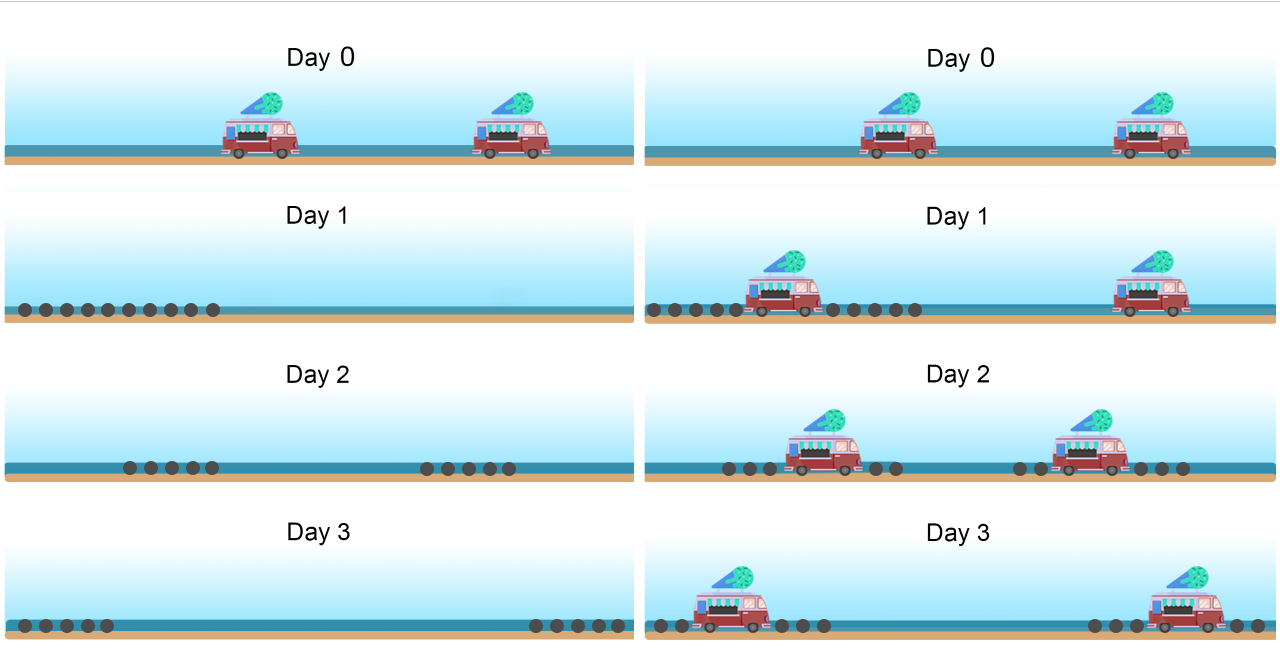
\includegraphics[scale=1.1]{chapters/previous_work/icecream.png}
\end{center}
\caption{Depiction of the simple example of Section~\ref{sec:prelim}. The picture on the left represents an instance of the $2$-Facility Reallocation problem on the line. The initial ice cream vendor locations are depicted in day 0 and the dots indicate the customer locations. On the right picture, we illustrate a good solution for this instance, namely the facility locations at each day.}
\label{example}
\end{figure}
The previous example is an instance of the $K$-Facility Reallocation problem, where the number of mobile facilities is two (the ice cream vendors), the number of stages is three (the days) and the number of agents is 10 (the customers). Moreover, the metric space is the real line (the beach) and the problem is  offline if we know all customer locations throughout the days at the beginning of the first day. The problem is online if we learn the customer positions of the next day only after we have served (located the ice cream vendors) the customers of the current day. The following definitions formalize these concepts. \\

The underlying assumption so far has usually been that the agent locations are known in advance, but this may not be the case in general. For example, in many natural settings such as network design or providing targeted content given preference clusters, the `agent locations' are not known in advance. Motivated by this fact, Meyerson~\cite{M2001} introduced online facility location problems, where agents arrive one-by-one and must be 
\emph{immediately and irrevocably} assigned to a facility upon arrival. Moreover, the set of agent locations is revealed in either random or adversarial order.  However, all connections are irrevocable and cannot be changed even if  new facilities are added, reflecting the constraints of adding physical links in a network. \\

More recently, understanding the dynamics of temporally evolving social or 
infrastructure networks has been the central question in many applied areas such 
as viral marketing, urban planning etc. Dynamic Facility Location 
proposed in similar versions by \cite{EMS2014} and \cite{fernandes2013dynamic} has been a new tool to analyze the temporal aspects 
of such networks. In this time dependent variant of facility location, the \emph{underlying metric space} can change over time. This can be perceived as agents moving through space, but is actually more flexible. Facilities cannot be moved around however: amongst the set of available facilities, the algorithm can select a subset to open at a cost. Then, at each turn, the assignment of agents to facilities can be changed. However, this incurs a \emph{switching cost} and the objective is to achieve the best tradeoff between the 
optimal connections of agents to facilities and the stability of solutions between  
consecutive timesteps. This switching cost can be interpreted differently depending on the situation modelled, but taking it into account can produce significantly different (and more `reasonable' looking) clusters than statically finding the best assignment each turn. \\

While the previous models have addressed issues of dynamically
maintaining a set of facilities (or clusters), the common theme has
been that facilities cannot move. They can be dissolved and reinstated
somewhere else, but the cost is usually measured in terms of active
facilities at the end. Our contribution is to study such settings where facilities can also \emph{move} around.

\subsection{Problem Definition and Preliminaries}
\label{sec:prelim}

\begin{definition}[\emph{$K$-Facility Reallocation problem}]\label{d:problem}
We are given a tuple $(x^0, C)$ as input. The $K$ dimensional vector 
$x^0=(x^0_1,\ldots,x^0_K)$
describes the initial positions of the facilities. The positions of the agents over 
time
are described by $C = (C_1, \ldots, C_T)$. The position of agent $i$ at stage $t$ 
is
$\alpha_i^t$ and $C_t = (\alpha_1^t, \ldots , \alpha_n^t)$ describes the 
positions 
of the agents at stage $t$.
\end{definition}


\begin{definition}\label{d:solution}
A solution to the K-Facility Reallocation problem is a sequence $x = (x^1, \ldots 
,x^T)$.
Each $x^t= (x_1^t,\ldots,x_K^t)$ is a $K$ dimensional vector that gives
the positions of the facilities at stage $t$ and
$x_k^t$ is the position of facility $k$ at stage $t$. The cost of the solution $x$ is
\[ \Cost(x) = \sum_{t=1}^{T} \bigg[\sum 
\limits_{k=1}^K|x_k^t-x_k^{t-1}|+\sum\limits_{i=1}^{n} \min_{1\leq k \leq 
K}|\alpha_i^t-x_k^t| \bigg].\]
\end{definition}
Given an instance $(x^0,C)$ of the problem, the goal is to find a solution $x$
that minimizes the $\Cost(x)$. The term 
$\sum_{t=1}^{T}\sum_{k=1}^K|x_k^t-x_k^{t-1}|$ describes
the cost for moving the facilities from place to place in a solution $x$. We  refer to it as 
\emph{moving cost} and is denoted as $\MovC(x)$. The 
 term $ \sum_{t=1}^{T}\sum_{i=1}^{n} \min_{1\leq k \leq K}|\alpha_i^t-x_k^t|$ 
describes the connection
cost of the agents in a solution $x$. We refer to it as \emph{connection cost} and is denoted as $\ConC(x)$. The connection cost of an agent $i$ at stage $t$ in solution $x$ is denoted as $\ConC_i^t(x)$ and is the quantity  $\min_{1\leq k \leq K}|\alpha_i^t-x_k^t|$. 

Observe that the competitive ratio of an online algorithm involves an additive constant $b$ in its definition. The additive constant may depend on the initial configuration of the problem (in our case the initial positions of the facilities) but not on the request sequence $\sigma$. This is the standard definition used in $K$-server like problems (see also \cite{KP95, BY1998}).

%\begin{remark}\label{r:convex}
%An interesting variant of the $K$-Facility Reallocation problem is when the objective function is of the form  $$ \sum_{t=1}^{T} \bigg[ \gamma \sum \limits_{k=1}^K   |x_k^t-x_k^{t-1}|+ (1-\gamma)\sum\limits_{i=1}^{n} \min_{1\leq k \leq 
%K}|\alpha_i^t-x_k^t| \bigg].$$ 
%where $\gamma \in [0, 1]$. The value of $\gamma$ determines if the connection cost accounts more than the moving cost or vice versa. This does not affect the performance of our offline algorithm. The competitive ratio of our online algorithm improves for $\gamma<1/2$ and worsens for $\gamma>1/2$. For $\gamma \rightarrow 1$ the competitive ratio becomes $O(\gamma)$.
%\end{remark}


\subsection{A Polynomial Time Algorithm for $K$-Facility Reallocation Problem}
\label{s:offline}



In this section, we present an algorithm which computes an optimal solution for the $K$-Facility 
Reallocation problem on the line with running time polynomial in  $n$, $T$ and $K$. Our approach is a typical LP based algorithm that consists of two basic steps.

\begin{itemize}
 \item \textbf{Step 1:} Expressing the $K$-Facility Reallocation problem as an Integer Program.
 \item \textbf{Step 2:} Solving \emph{fractionally} the relaxation of the  Integer Program and 
 \emph{rounding} the fractional solution to an integral one.
\end{itemize}

The main technical contribution is showing that a simple rounding 
scheme yields an integral solution
that has the exact same cost with an optimal
fractional solution.


\subsection{Presentation of the offline algorithm}
We start by expressing the $K$-Facility Reallocation problem on the line as 
an Integer Program. The following lemma from \cite{KW2018} suggests that we can focus on finite locations on the real line.




\begin{fact}[Lemma~2 in \cite{KW2018}] \label{l:discrete}
Let $(x_0,C)$ be an instance of the $K$-Facility Reallocation problem.
There exists an optimal solution $x^*$ such that for all stages
$t \in [T]$ and $k \in \{1, \ldots ,K\}$,
\[x_k^{*t} \in C_1 \cup \ldots \cup C_T \cup x^0 .\]
\end{fact}

According to Fact~\ref{l:discrete}, there exists an optimal solution that places 
the facilities only at locations where either an agent has appeared or a facility 
was initially lying. This allows us to focus only on solutions which place facilities on at most $K+Tn$ different locations on the real line.
Fact~\ref{l:discrete} provides an exhaustive search algorithm for the problem 
and is also the basis
for the \emph{Dynamic Programming} approach in \cite{KW2018}, which has running time $O(T^2(\max \{Tn,k \})^{k+1})$. We will use 
Fact~\ref{l:discrete} to formulate our Integer Program.



Specifically, let $\mathrm{Loc} \coloneqq C_1 \cup \ldots \cup C_T \cup x^0$ denote the set of the  locations of Fact~\ref{l:discrete}. This set can be equivalently represented by a \emph{locations path} $P = (V,E)$. That is, if we sort the locations of $\mathrm{Loc}$ in non decreasing order, then the $j$th location of $\mathrm{Loc}$ is the $j$th node of the locations path $P$ and the distance between two nodes in $P$ is the distance of the corresponding locations on the line.
% That is, we sort the locations of $\mathrm{Loc}$ and the $j$th node of the positions path $P$ is the 
% In this path, the $j$th node corresponds to the $j$th leftmost position of $\mathrm{Pos}$ 
% and the distance between two consecutive nodes on the path equals the 
% distance of the respective positions on the real line.
Now, the $K$-Facility Reallocation problem on the line takes the following 
\emph{discretized form}:
For an instance $(x^0,C)$, we can construct a locations path $P = (V,E)$.
Each facility is initially located at a node $j \in V$ and at each stage $t$, 
each agent is also located at a node of $P$.
The goal is to move the facilities from node to node such that the connection 
cost of the agents plus the moving cost
of the facilities is minimized.

To formulate this discretized version as an Integer Program,
we introduce some additional notation. Let $\dist(j,l)$ be the distance of the nodes 
$j,l \in V$ in $P$ and $A$ be the set of agents. For each $i \in A$, $\Loc(i,t)$ is the node 
where agent $i$ is located at stage $t$.
We also define the following $\{0,1\}$-indicator variables for all $t\in [T] $:
$\zeta_{ij}^t =1$ if, at stage $t$, agent $i$ connects to a facility located at node $j$,
$f_{kj}^t =1$ if, at stage $t$, facility $k$ is located at node $j$,
$S_{kjl}^t =1$ if facility $k$ was at node $j$ at stage $t-1$ and moved to node 
$l$ at stage $t$. The variable $c_j^t$ represents the number of facilities that are placed on node $j$ at stage $t$. 
This problem can be formulated as the Integer Program depicted in 
Figure~\ref{LP_Reallocation}.

 
\begin{figure}
\centering
$
\text{minimize}\sum _{t=1}^T \bigg[ \sum\limits_{i\in 
  C}\sum\limits_{j\in V} \dist(\Loc(i,t),j)\zeta_{ij}^t + \sum\limits_{k\in F} S_k^t \bigg] $
$
\begin{array}{lr}
\\\\
(1) \,\,\,\,\,\,  \sum \limits_{j \in V}\zeta_{ij}^t=1  &\forall i \in A,t \in [T]  \\\\
(2) \,\,\,\,\,\,	\zeta_{ij}^t \leq c_j^t&\forall i \in A,j \in V,t \in [T]\\\\
(3) \,\,\,\,\,\,     c_j^t=\sum\limits_{k=1}^{K} f_{kj}^t & \forall j \in V, t\in [T]\\\\
(4) \,\,\,\,\,\,    \sum \limits_{j \in V} f_{kj}^t=1 & \forall k\in [K], t\in [T]\\\\
(5) \,\,\,\,\,\,        S_k^t = \sum \limits_{j,l \in V} \dist(j,l)S_{kjl}^t & \forall k \in [K], t\in [T] \\\\
(6) \,\,\,\,\,\,        \sum \limits_{j \in V} S_{kjl}^t =f_{kl}^t & \forall l \in V,k \in [K],t\in [T]\\\\
(7) \,\,\,\,\,\,       \sum \limits_{l \in V} S_{kjl}^t = f_{kj}^{t-1} & \forall j \in V,k \in [K],t\in [T]\\\\
(8) \,\,\,\,\,\,        \zeta_{ij}^t,f_{kj}^t,S_{klj}^t \in \{0,1 \} & \forall j \in V,k \in [K],t\in [T]\\\\
\end{array}
$
\caption{Integer Program formulation of the K-\text{Facility Reallocation problem} }
\label{LP_Reallocation}
\end{figure}

Constraints (1)-(4) of the Integer Program are the standard $K$-median constraints with the only difference that the  facilities are distinguished, each having a different label. Facility $m$ is the $m$th leftmost facility according to the initial facility locations ordered from left to right. Constraints (5)-(7) describe a flow problem and are used to model the moving cost incurred by the movement of facilities between stages.
Specifically, constraints (1)-(3) correspond to the fact that at every stage $t$, each 
agent $i$ must be connected
to a node $j$ where at least one facility $k$ is located.
The constraint $\sum_{j \in V} f_{kj}^t=1$ enforces each facility $k$ to be located 
at exactly one node $j$.
The constraint $S_k^t = \sum_{j,l \in V} \dist(j,l)S_{kjl}^t$ describes the cost for 
moving facility $k$ from node $j$ to node $l$.
Constraints (6)-(7) ensure that facility $k$ moved from node $j$ to node 
$l$ at stage $t$ if and only if
facility $k$ was at node $j$ at stage $t-1$ and was at node $l$ at stage $t$
($S_{kjl}^t = 1$ iff $f_{kl}^t=1$ and $f_{kj}^{t-1}=1$). 
Observe that the values of $f_{kj}^0$ are determined by the initial positions
of the facilities, which are given by the instance of the problem. 

For ease of exposition, we will refer to the Integer Program of the $K$-Facility Reallocation problem as $\IPR$ and we will refer to the relaxation of the $\IPR$ as  $\LPR$. An optimal fractional solution of the $\LPR$ is denoted as $\ZLP$.


\begin{algorithm}[t]
    \caption{Algorithm for the offline case}\label{alg:offline}
    \textbf{Input:} The initial positions $x^0 = \{x_1^0,\ldots,x_K^0\}$ of the facilities and
    the positions of the agents $C = \{C_1,\ldots,C_T\}.$
    \begin{algorithmic}
        \STATE Construct the path $P$ and the $\IPR$~(Figure \ref{LP_Reallocation}).
        \STATE Solve the relaxation $\LPR$ of the $\IPR$.
        \FOR{each stage $t\geq 1$:}
            \FOR{$m=1,\ldots,K$, find the node  $j_m^t$ such that $\sum_{\ell = 1}^{j_m^t -1}c_\ell^t \leq m-1 < \sum_{\ell = 1}^{j_m^t}c_\ell^t$} 
                \STATE Locate facility $m$ at the respective location $x_m^t$ the 
  line, namely $x_m^t \leftarrow \dist(j_m^t,1) + \min_{p \in C_1 \cup \ldots \cup C_T \cup x^0}
  p.$
            \ENDFOR
        \ENDFOR
    \end{algorithmic}
\end{algorithm}

Our algorithm, described in Algorithm~\ref{alg:offline}, is a simple rounding scheme of an optimal fractional solution $\ZLP$ for the $\LPR$. At each stage $t$, the rounding procedure starts from the first node from the left and
finds for each facility $m$, $1\leq m \leq K$, the sum of the total facility amount placed on the visited nodes until a node $j_m^t$ makes this sum greater than $m-1$. Then, the algorithm places facility $m$ to the location on the line, which corresponds to node $j_m^t$. Observe, that this procedure leads to a placement of the facilities on the leftmost position of their fractional appearance ($f_{kj}>0$) in $\ZLP$ at each stage.       

Our goal is to show that the aforementioned rounding scheme produces an integral solution that has the exact same cost with $\ZLP$. The next section is dedicated to highlight the core ideas and basic steps of this fact.




\subsection{Overview of our approach }
In this section, we discuss the core ideas and basic steps for proving that Algorithm~\ref{alg:offline}
provides an optimal solution for the $K$-Facility Reallocation problem on the line. Our goal is to show the following theorem. 




\begin{theorem}~\label{l:main_stageing}For the $\LPR$, there exist $N$ integral solutions $\Sol_p$, $1\leq p \leq N$, for some integer $N>0$, such that:
\begin{itemize}
    \item $\frac{1}{N}\sum_{p=1}^N\ConC_i^t(\Sol_p)=\sum_{j\in V} 
    \dist(\Loc(i,t),j)\zeta_{ij}^t$ \,\,\, (1)
    \item $\frac{1}{N}\sum_{p=1}^N\MovC(\Sol_p)=\MovC(\ZLP)$ \,\,\,\,\,\, \,\,\, \,\,\,\,\,\,\,\,\,  (2)
\end{itemize}
Furthermore, the solution produced by Algorithm~\ref{alg:offline} is one of the $N$ integral solutions $\Sol_p$, $1\leq p \leq N$.
\end{theorem}


Theorem~\ref{l:main_stageing} directly implies that the total cost of each integral solution $\mathrm{Sol}_p$ equals the cost of the optimal fractional solution $\mathrm{Z_{LP}}$. Unfortunately, the number $N$ of the integral solutions $\Sol_p$ can be exponential with respect to the parameters of the problem, thus producing all of them is not an option.
However, we will show that the rounding scheme of Algorithm~\ref{a:1}, 
which clearly runs in polynomial time with respect to $n, K$ and $T$, produces one of these solutions, namely $\Sol_1$. 


The fact that each integral solution $\Sol_p$, $1 \leq p \leq N$, has the same cost with an optimal fractional solution follows easily from Theorem~\ref{l:main_stageing}.
Observe that by taking a sum over all clients and all stages in the first equation of Theorem~\ref{l:main_stageing}, we have that the average connection cost of the solutions $\Sol_p$ equals the connection cost of $\ZLP$. Combining this result with the second equation of Theorem~\ref{l:main_stageing}, we have that the solutions $\Sol_p$ have average cost equal to the optimal fractional cost, i.e., $\frac{1}{N} \sum_{p=1}^{N}\Cost(\Sol_p)= \Cost(\ZLP)$. Since $\Cost(\Sol_p) \geq  \Cost(\ZLP)$ for every $p$, $1\leq p \leq N$, it must hold that $\Cost(\Sol_p)= \Cost(\ZLP)$ for every $p$, $1\leq p \leq N$. 


Due to technical and intuitive reasons, we break down the proof of Theorem~\ref{l:main_stageing} into two steps. In the first step, which we exhibit in Section~\ref{s:semi_integral}, we prove that Theorem~\ref{l:main_stageing} holds if we further assume that the values of the variables in an optimal fractional solution are either $1/N$ or $0$. Formally,

\begin{assumption}\label{a:1}
There exists a positive integer $N$, such that the  variables $f_{kj}^t$ and $c_j^t$ of the $\LPR$ have value either $1/N$ or $0$.
\end{assumption}
\noindent

We use Assumption~\ref{a:1} to define the integral solutions $\Sol_p$ that are the main component of our proofs. Each solution $\Sol_p$ places facilities on a subset of nodes with positive $c_j^t$.

\begin{definition}\label{d:positive}
$V_t^{+}$ denotes the set of nodes of the locations path $P$ with a positive amount of facility 
($c_j^t$) at stage $t$,
\[j \in V_{t}^+ \iff c_j^t = 1/N \,.\]
\end{definition}

\noindent We remind that since $c_j^t$ is either  $1/N$ or $0$ then $|V_t^+| = K \cdot N$. We 
also consider the nodes in $V_t^{+} = \{Y_1^t,\ldots,Y_{K \cdot N}^t\}$ to be 
ordered from left to right. Now, we can formalize the concept of the solutions $\Sol_p$, which will be used throughout the proofs. The term $m$th facility in the following definition of the integral solutions $\Sol_p$ refers to the ordering of the facilities on the real line according to their initial locations $\{x_1^0, \ldots ,x_K^0 \}$.

\begin{definition}\label{def:Sol_p}
$\Sol_p$ denotes the integral solution that at each stage $t$ places the $m$th facility 
at the $(m-1)N + p$ node of $V_t^+$
,i.e., $Y_{(m-1)N + p}^t$, where $1\leq p \leq N$. 
\end{definition}

\noindent Since the solutions $\Sol_p$ play an important role in the understanding of the proof details, we provide an example of their structure in Figure~\ref{fig:Sol_p}. 
% Observe that the solution provided by Algorithm~\ref{alg:offline} corresponds to $\Sol_1$.

\begin{observation}\label{o:sol_1}
$\Sol_1$, which is the integral solution that at each stage $t$ places the $m$th facility 
at node $Y_{(m-1)N + 1}^t$, is the solution produced by Algorithm~\ref{alg:offline}.
\end{observation}

Since Algorithm~\ref{alg:offline} provides one of the solutions $\Sol_p$, it remains to show the two claims of Theorem~\ref{l:main_stageing}. We start by demonstrating the high-level idea for the proof of the first claim.

\begin{figure}
    \centering
    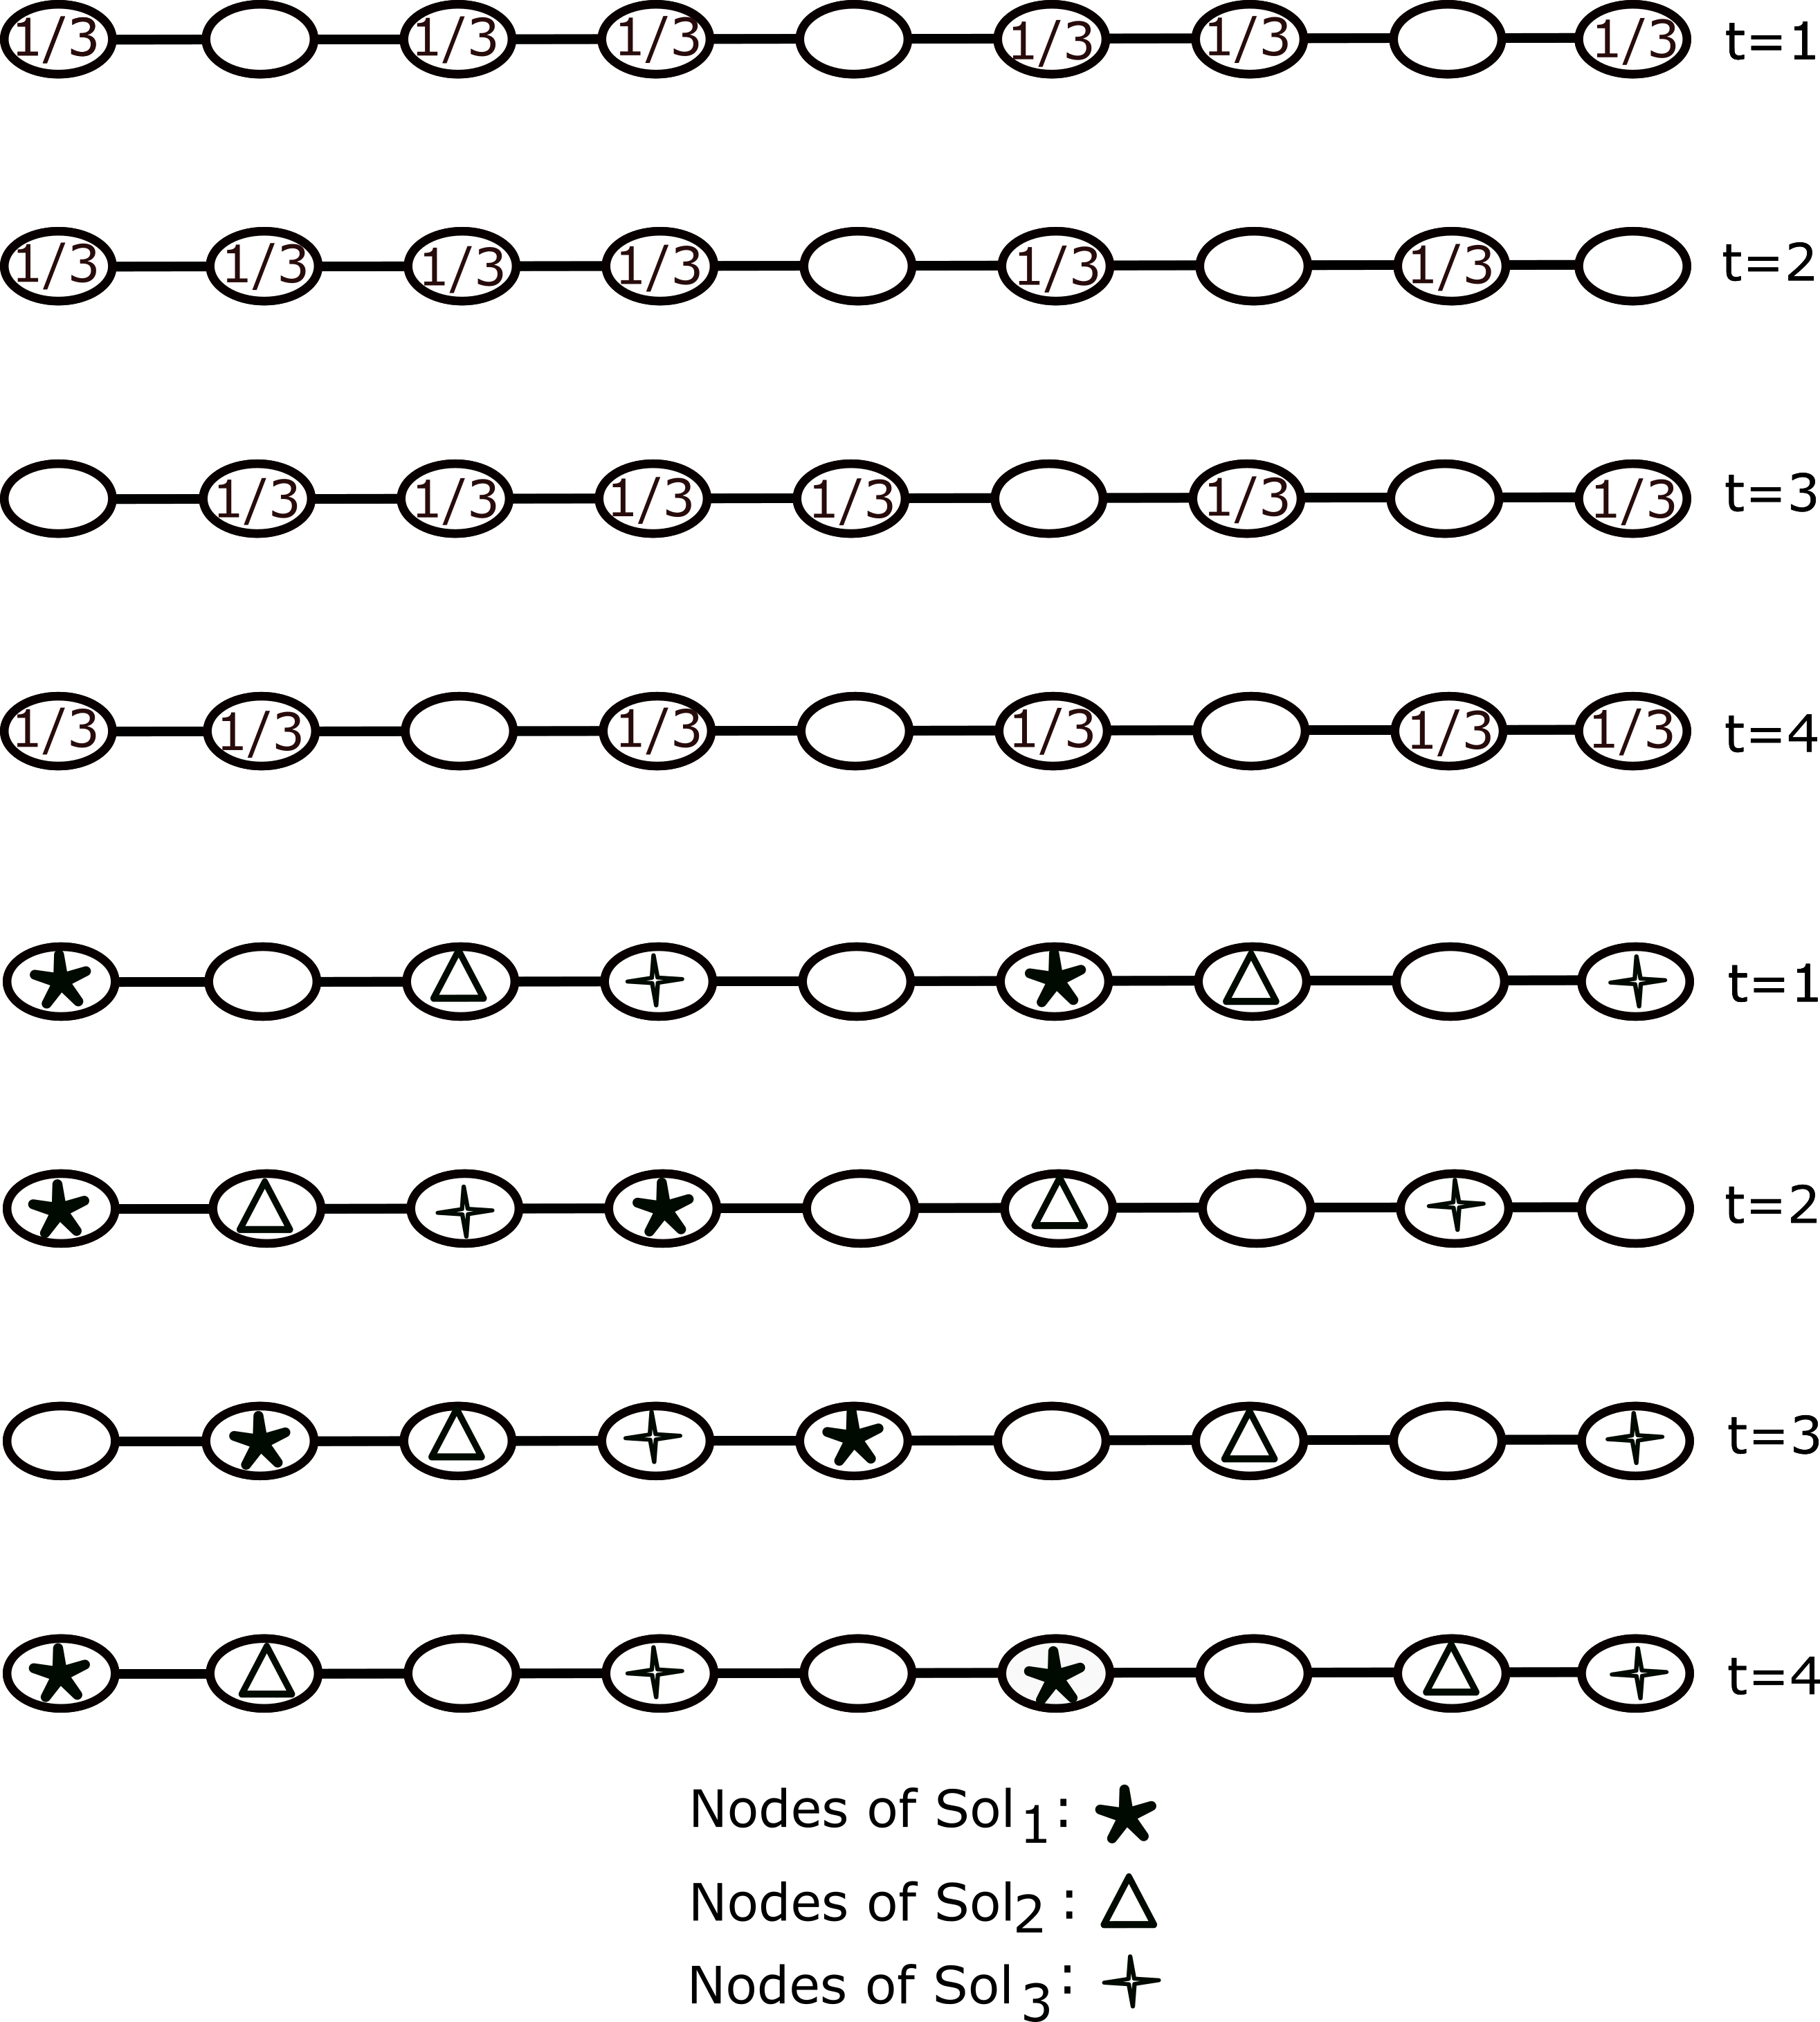
\includegraphics[scale=0.14]{Sol_p.png}
    \caption{The figure above is a graphical illustration of the optimal fractional solution $\ZLP$ (top) together with the integral solutions $\Sol_p$ (bottom). For this instance $N=3, T=4$ and $K=2$. $\ZLP$ puts $1/N=1/3$ amount of facility on some nodes at each stage. These nodes are the nodes of $V_t^+$, $1 \leq t \leq T$, which are grouped in $K=2$ blocks with $N=3$ nodes each ( $|V_t^+|=6$). Starting from the left, $Sol_1$ (asterisk) puts the two facilities  on the first node of each block of $V_t^+$, $Sol_2$ (triangle) puts the two facilities on the second node of each block of $V_t^+$ and $Sol_3$ (cross) puts the two facilities on the third node of each block of $V_t^+$, at each stage $t$. $Sol_1$ is the solution, which  Algorithm~\ref{alg:offline} produces for this instance.}
    \label{fig:Sol_p}
\end{figure}

% Let $V_{t}^+$ denote the nodes of the locations path $P$, which have an amount of $c_j^t=1/N$ at stage $t$. Then, the solution $\Sol_p$ puts the $m$th facility on the node $(m-1)N+p$ of $V_t^+$. It is easy to see that the solution provided by Algorithm~\ref{alg:offline} corresponds to the integral solution $\Sol_1$. For a graphical illustration of the solutions $\Sol_p$, you can see Figure~\ref{fig:Sol_p}.


The core idea of the proof is that agent $i$ connects to $N$ nodes in $\ZLP$, on which the $N$ distinct solutions $Sol_p$ have placed a facility, at stage $t$. Specifically, $i$ finds the $N$ closest nodes $N_i^t$ of $V_t^+$ in $\ZLP$ and receives $1/N$ amount of service from each facility on these nodes. The nodes of $N_i^t$ are consecutive nodes of $V_t^+$. By the construction of the solutions $\Sol_p$, there exists a unique node in $N_i^t$ where each $\Sol_p$ places a facility. 
% Meaning that the nodes of $N_i^t$ which $i$ connects in $\ZLP$ are $\{Y_{j\cdot N + 1}^t, \ldots, Y_{j\cdot N + N }^t \}$, where each of the $N$ solutions $\Sol_p$ have a facility. 
Thus, the average connection cost of $i$ in the integral solutions is the same with the connection cost of $i$ in $\ZLP$ at stage $t$. We illustrate these ideas Figure~\ref{fig:ConCost} and present the formal proof in Lemma~\ref{l:connection_cost}.

\begin{figure}[t]
    \centering
    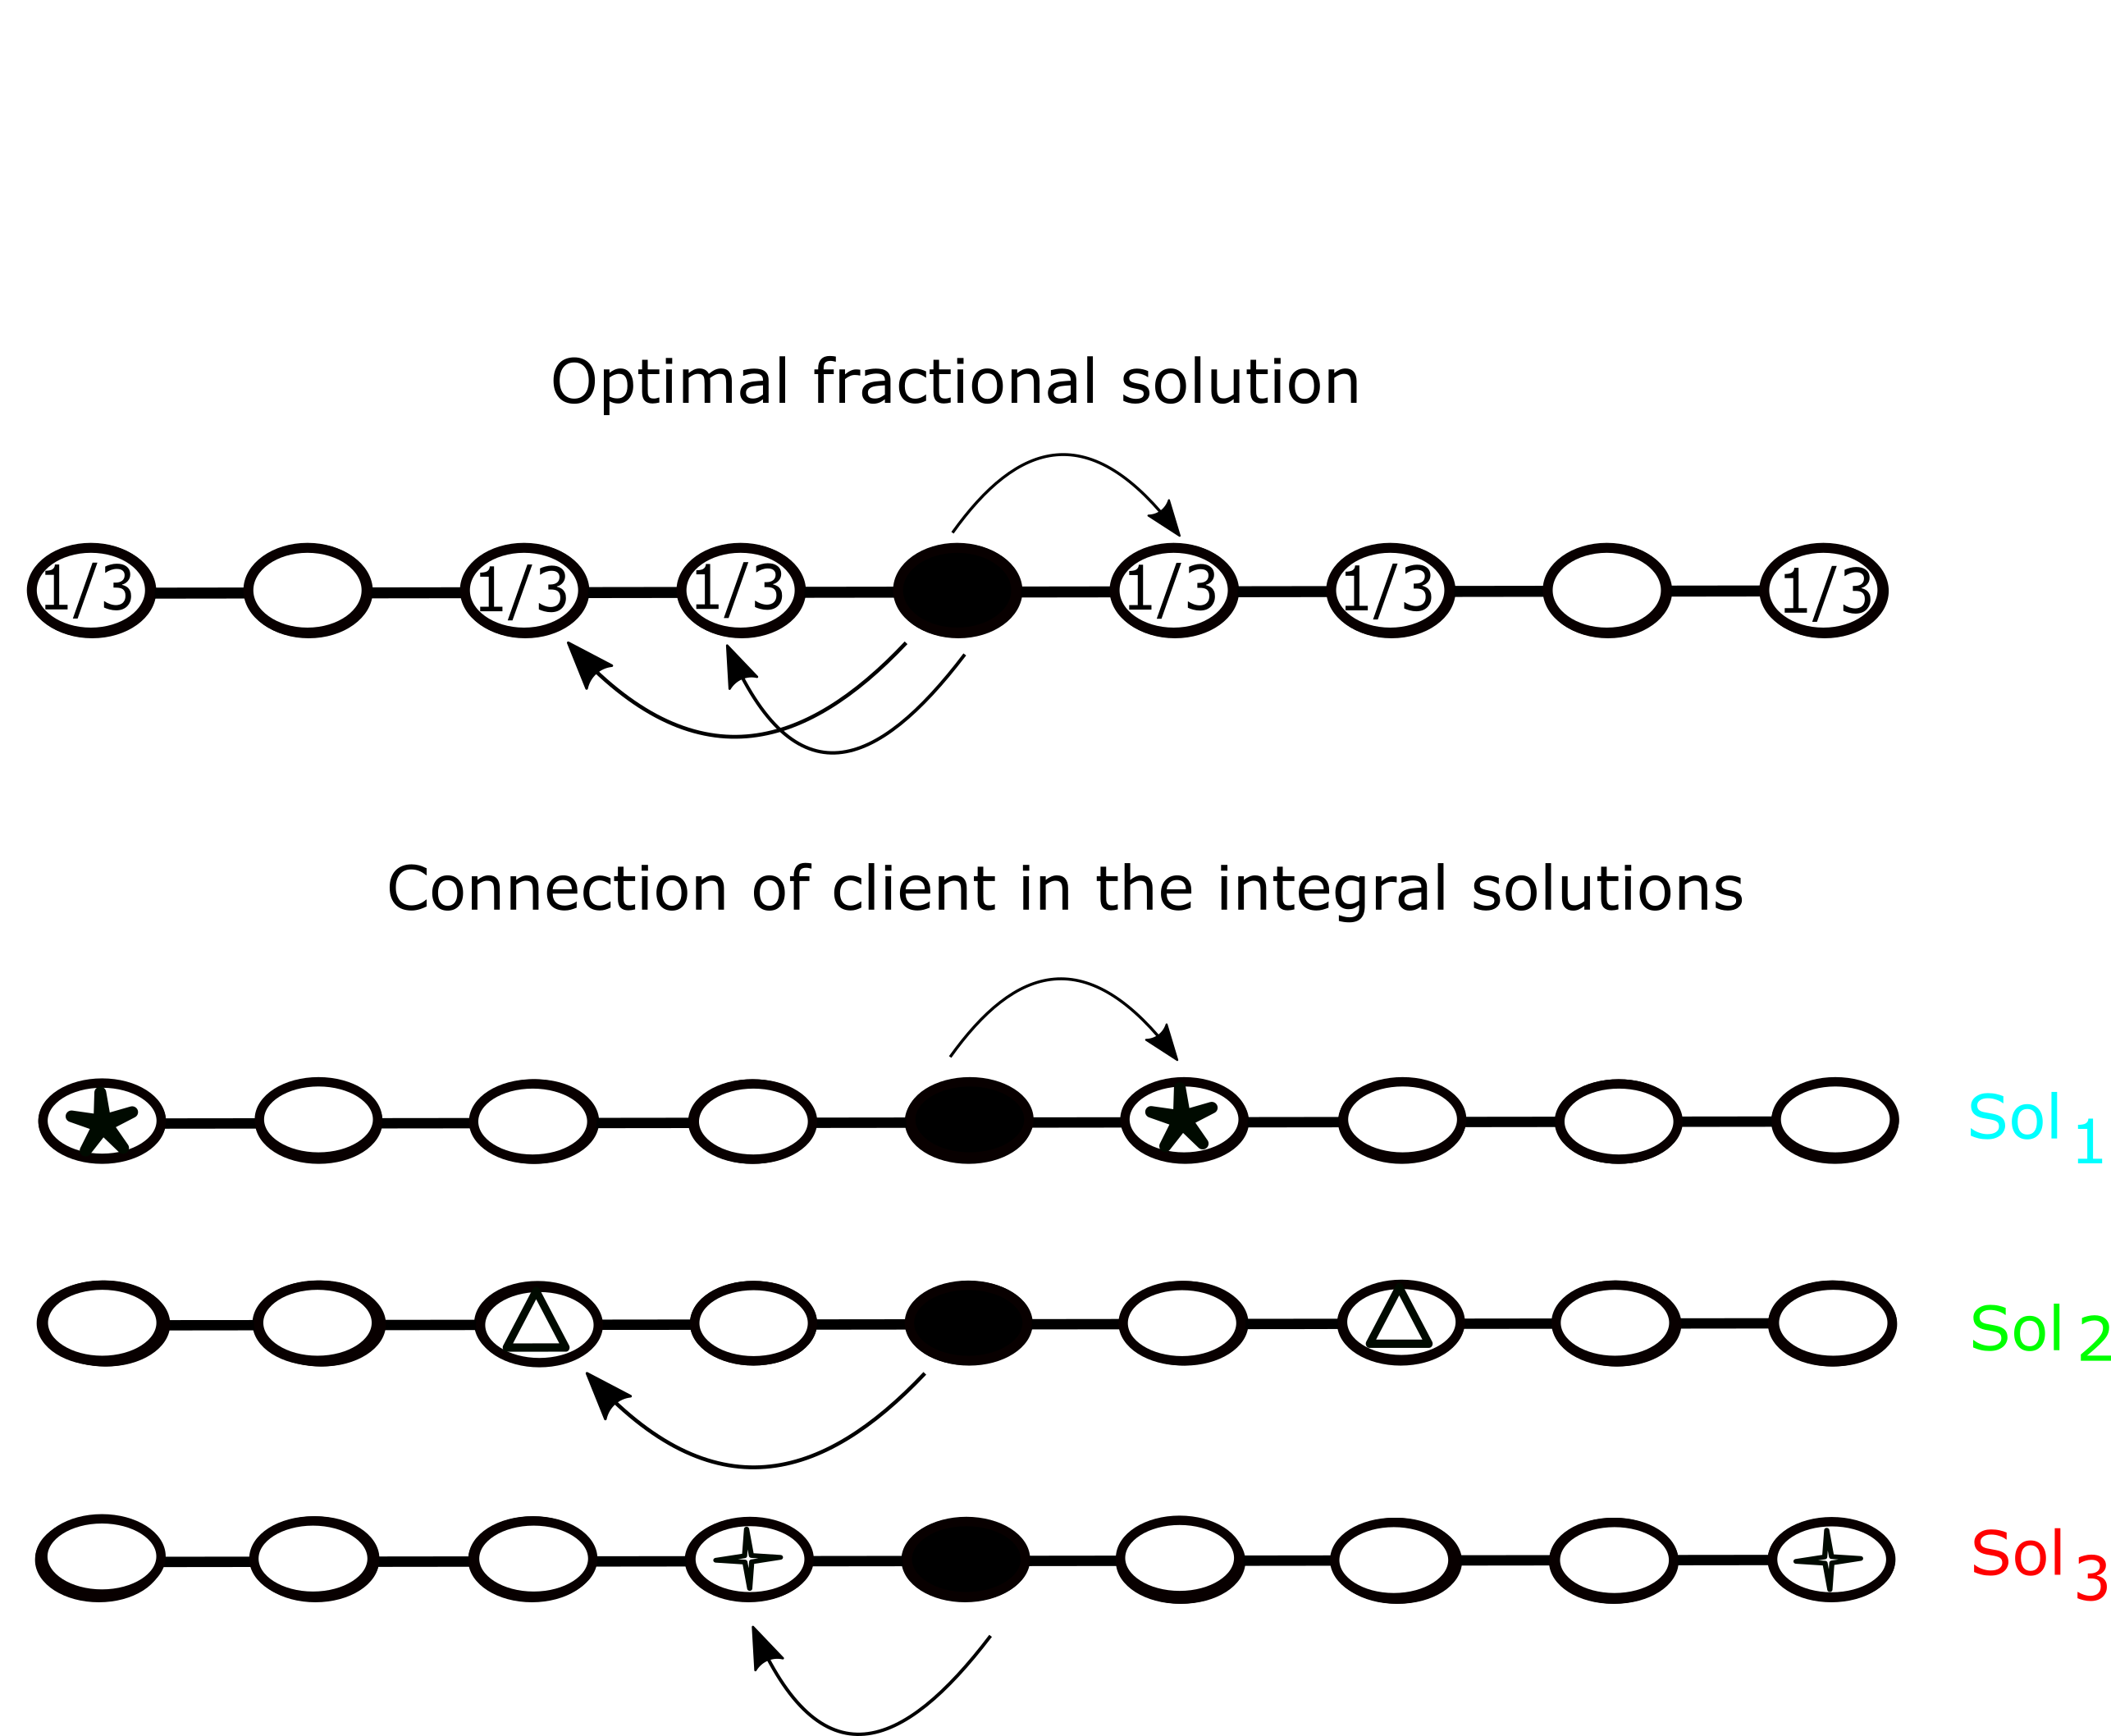
\includegraphics[scale=0.14]{connectioncost.png}
    \caption{In this example, we illustrate the relation of the integral solutions $\Sol_p$ with the optimal fractional solution $\ZLP$ in terms of connecting agents. We have 2 facilities ($K=2$), $N=3$ and an agent $i$ on the  5th node (with black color) from the left. The figure on the top depicts the placement of the $\zeta_{ij}^t=1/N=1/3$ amount in $\ZLP$, where $i$ receives $1/3$ amount of service from his $N$ closest facilities. The figure on the bottom shows the connection of the same agent in the integral solutions $\Sol_1, \Sol_2$ and $\Sol_3$.}
    \label{fig:ConCost}
\end{figure}

% Next, we present the main ideas and basic steps for proving the second claim of Theorem~\ref{l:main_stageing} under Assumption~\ref{a:1}, namely that the average moving cost of the solutions $\Sol_p$ is equal to the optimal fractional moving cost.



The key idea for proving the second claim of Theorem~\ref{l:main_stageing} resides again on the structure of the solutions $\Sol_p$.
Assume that the optimal fractional solution $\ZLP$ places positive $1/N$ amounts of facility $m$ on $N$ nodes of $V_{t-1}^+$ at stage $t-1$. Then, this set of nodes $N^{t-1}$ are consecutive nodes of $V_{t-1}^+$ and each $\Sol_p$ places facility $m$ on a unique node of $N^{t-1}$. By solving a flow problem, we show that the optimal fractional solution moves the $1/N$ amounts of facility $m$ to the nodes $N^{t}$ of $V_{t}^{+}$ in the same way that the solutions $\Sol_p$ move the facility $m$ to a node of $N^{t}$. Thus, if $\ZLP$ moves $1/N$ amount of facility $m$ from node $j_{t-1} \in N^{t-1}$ to node $j_t \in N^{t}$, there is a unique solution $\Sol_p$ that moves facility $m$ from $j_{t-1}$ to $j_{t}$.
% Meaning that $\ZLP$ moves $1/N$ amounts of facility $m$ from nodes $\{Y_{(m-1)\cdot N + 1}^t, \ldots, Y_{(m-1)\cdot N + 
% p}^t \}$ at stage $t-1$ to nodes $\{Y_{(m-1)\cdot N + 1}^t, \ldots, Y_{(m-1)\cdot N + 
% N}^t \}$ at stage $t$, and $\Sol_p$ move fractions from nodes $\{Y_{(m-1)\cdot N + 1}^t, \ldots, Y_{(m-1)\cdot N + 
% N}^t \}$
Summing over all facilities and stages, we get that the average moving cost paid by the solutions $\Sol_p$ is the same with the moving cost of the optimal fractional solution. The idea behind this proof is depicted in Figure~\ref{fig:movingcost}. The formal proof is presented in Lemma~\ref{l:moving_cost}.


\begin{figure}
    \centering
    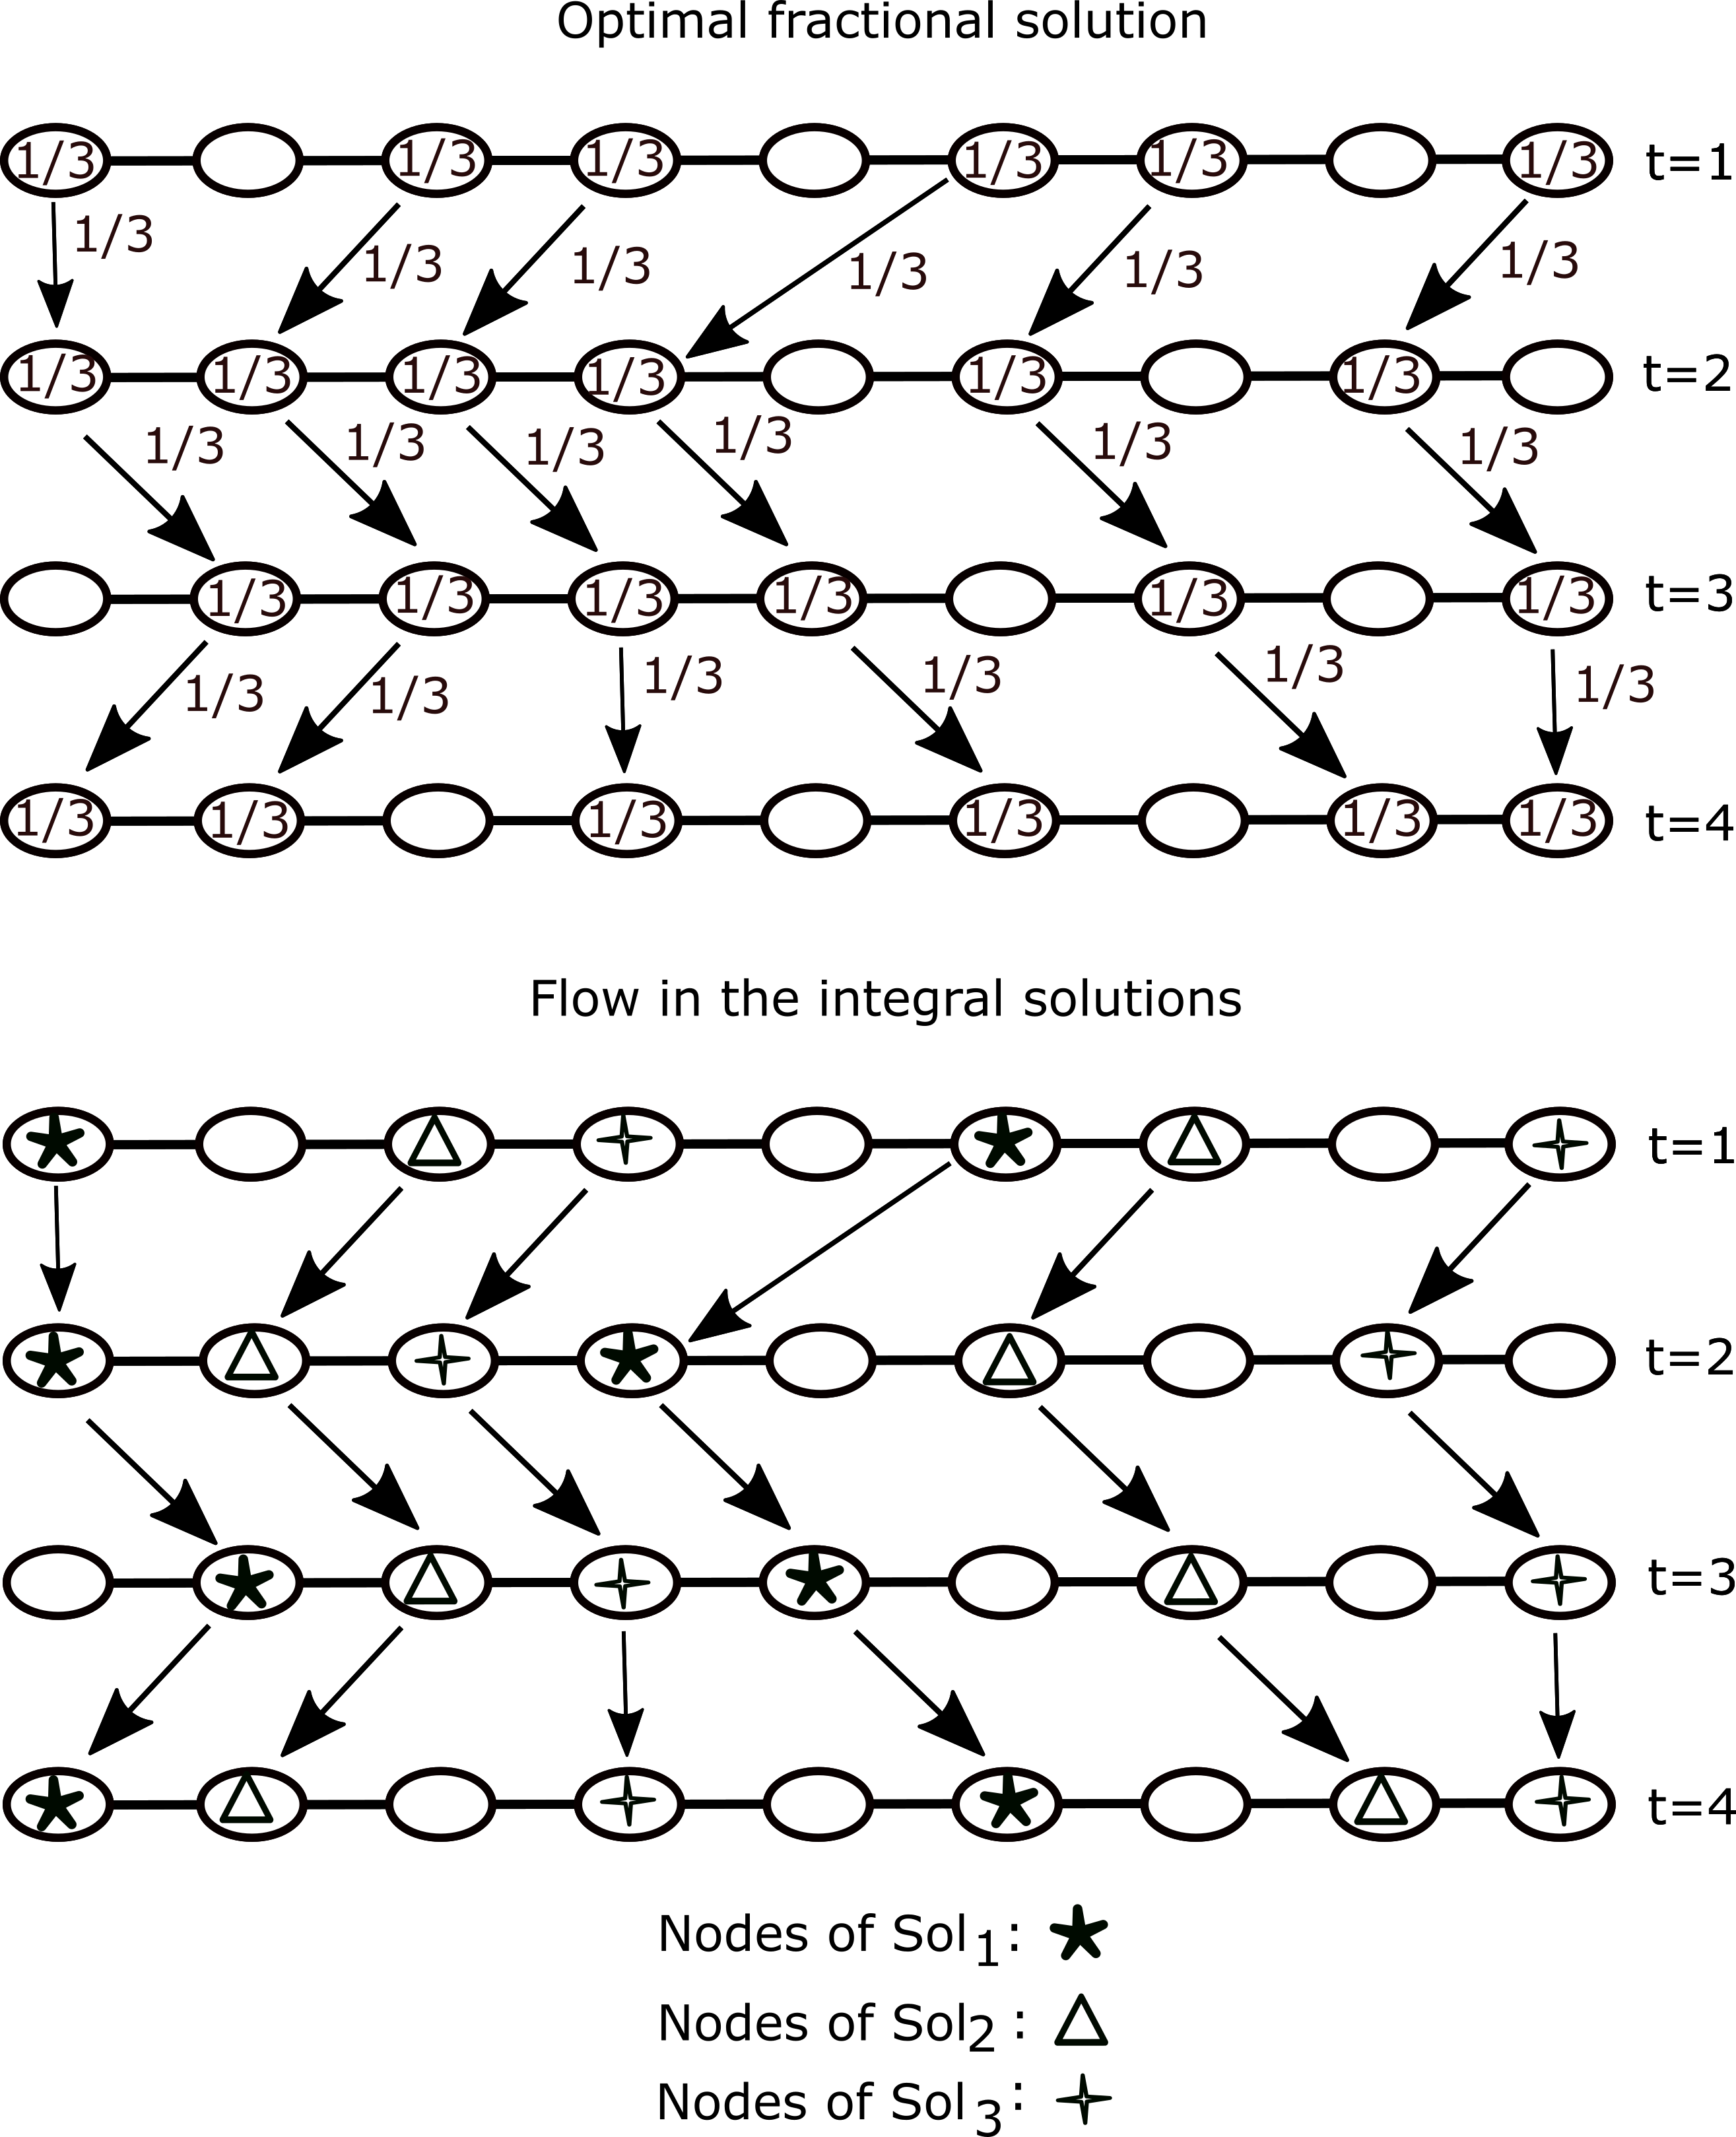
\includegraphics[scale=0.14]{moving_cost.png}
    \caption{In this example, we illustrate the relation of the integral solutions $\Sol_p$ with an optimal fractional solution $\ZLP$ in terms of moving facilities. We have 2 facilities ($K=2$) and $N=3$. The top figure depicts an instance where $\ZLP$ has placed $1/N=1/3$ amount of facility on some nodes in the locations path $P$. We show in Lemma~\ref{l:moving_cost} that $\ZLP$ sends these positive fractions of facilities to nodes of the next stage as depicted by the arrows. The bottom figure illustrates how $\Sol_1, \Sol_2$ and $\Sol_3$ move facilities between stages. Observe that each facility is moved to the same node that has moved it's corresponding fraction in $\ZLP$.}
    \label{fig:movingcost}
\end{figure}



The second step for proving Theorem~\ref{l:main_stageing} is presented in Section~\ref{s:rounding_general}, where we show how to generalize the result of Section~\ref{s:semi_integral} for an optimal fractional solution that does not satisfy Assumption~\ref{a:1}. Assume that we have such an optimal fractional solution $\ZLP$ of the $\LPR$ in the locations path $P$. From this solution, we can construct an optimal fractional solution $\ZLPO$ of the $\LPR$ in a path $P'$ that satisfies Assumption~\ref{a:1}. $P'$ is constructed from the locations path $P$ by splitting each node in $KN$ copies of zero distance. Then, in Lemma~\ref{l:construction} we show that $\ZLP$ and $\ZLPO$ have the same cost. 

We conclude Section~\ref{s:offline} by providing 
the proof of Theorem~\ref{l:main_stageing}. By the construction of path $P'$, it is easy to see that the solutions $\Sol_p$ correspond to $\Sol_p^*$ in the original locations path $P$ with the same connection and moving cost. Since Theorem~\ref{l:main_stageing} holds for the solutions $\Sol_p$ and $\Cost(\ZLP)=\Cost(\ZLPO)$, both claims of Theorem~\ref{l:main_stageing} hold also for the solutions  $\Sol_p^*$. Finally, $\Sol_1^*$ is the solution produced by Algorithm~\ref{alg:offline} therefore  Theorem~\ref{l:main_stageing} holds in the general case.

% Since we have already shown in the previous section that 
% we prove that we can transform it to a fractional solution $\ZLP$ of the $\LPR$, which has the same cost and satisfies Assumption~\ref{a:1}. Since we have already proven Theorem~\ref{a:1} for $\ZLP$, it holds also for the generic solution $\ZLPP$.

\begin{remark}\label{r:extreme_point}
An optimal solution for the $K$-Facility Reallocation problem on the line can be computed by finding an optimal extreme point for the $\LPR$ and by proving that this extreme point will be integral.
However, proving Theorem~\ref{l:main_stageing} serves our end and provides better exposition and brevity.
\end{remark}





\subsection{Proving Theorem~\ref{l:main_stageing} under Assumption~\ref{a:1}}
\label{s:semi_integral}
Throughout this section, we assume that Assumption~\ref{a:1} is satisfied; 
$f_{k j}^t$ and $c_j^t$ are either $1/N$ or $0$ , for some positive integer $N$.  

The following lemma states that the average connection cost an agent pays in an integral solution $\Sol_p$, at each stage $t$, is the same with the connection cost that he pays in an optimal fractional solution at each stage $t$.  


\begin{lemma}\label{l:connection_cost}
 For an agent $i$ at stage $t$, under Assumption~\ref{a:1} it holds that
\[\frac{1}{N}\sum_{p=1}^N \ConC^t_i(\Sol_p) =\sum_{j\in V} 
\dist(\Loc(i,t),j)\zeta_{ij}^t
.\]
\end{lemma}
\begin{proof2} By Assumption~\ref{a:1}, $c_j$ is $1/N$ if $j \in V_t^+$ and $0$ 
otherwise. As a result, in an optimal fractional solution, each agent $i$ finds the 
$N$ closest to $\text{Loc}(i,t)$ nodes of $V_t^+$ and receives a $1/N$ amount 
of service from each one of them.
Let us call this set $N_i^t$. Then, the 
nodes in $N_i^t$ are consecutive nodes of $V_t^+$ i.e. $N_i^t = 
\{Y_l^t,\dots,Y_{l+N-1}^t\}$ and since $\sum_{j \in V}\zeta_{ij}^t = 1$ we have that
\[\sum\limits_{j\in V} \dist(\text{Loc}(i,t),j)\zeta_{ij}^t =  \sum\limits_{j = l}^{l+N-1} 
\dist(\text{Loc}(i,t),Y_j^t)/N.\]

% Let an agent $i$ that at some stage $t$ has $\zeta_{i Y_j^t}^t>0,\zeta_{i Y_\ell^t}^t< 
% 1/N$ and $\zeta_{i Y_h^t}^t > 0$ for some $j < \ell < h$. Assume that $\text{Loc}(i,t) 
% \leq Y_\ell^t$ and to simplify notation consider $\zeta_\ell = \zeta_{i Y_\ell^t }^t,\zeta_h = 
% \zeta_{i Y_h^t }^t $.
% Now, increase $\zeta_\ell$ by $\epsilon$ and decrease $\zeta_h$ by $\epsilon$, where 
% $\epsilon = \min(1/N - \zeta_\ell,\zeta_h)$. Then, the cost of the solution is decreased by 
% $(\dist(\text{Loc}(i,t),h) - \dist(\text{Loc}(i,t),\ell))\epsilon > 0$, thus contradicting the 
% optimality of the solution. The same argument holds if $\text{Loc}(i,t) \geq 
% Y_\ell^t$. The proof follows since 
% $\sum_{j \in V}\zeta_{ij}^t = 1$.

\noindent Since $\Sol_p$ puts facilities in the positions $\{Y_{(m-1)\cdot N + 
p}^t\}_{m=1}^K$,
there exists a unique node $Y_{l(p)}^t \in N_i^t$ on which $\Sol_p$ puts a facility.
$Y_{l(p)}^t$ is the closest node to $\text{Loc}(i,t)$ from all the nodes in which 
$\Sol_p$ puts a facility.
As a result, $\ConC_i^t(\Sol_p)= \dist(\text{Loc}(i),Y_{l(p)}^t)$. Now, summing  
over $p$ we get,
\begin{align*}
\frac{1}{N}\sum\limits_{p=1}^N \ConC_i^t(\Sol_p) &= 
\frac{1}{N}\sum\limits_{p=1}^N \dist(\text{Loc}(i),Y_{l(p)}^t)\\
&= \sum\limits_{j=l}^{l+N-1} \dist(\text{Loc}(i),Y_j^t)/N\\
&=\sum\limits_{j\in V} \dist(\text{Loc}(i,t),j)\zeta_{ij}^t.
\end{align*}
\end{proof2}
\medskip

\noindent
The proof of Lemma~\ref{l:connection_cost} establishes the first claim (1) of Theorem~\ref{l:main_stageing}.
The next step is to prove that the average moving cost of the integral solutions $\Sol_p$ is the same with the moving cost of $\ZLP$. This is formally stated in the following lemma.



% \begin{figure}
%     \centering
%     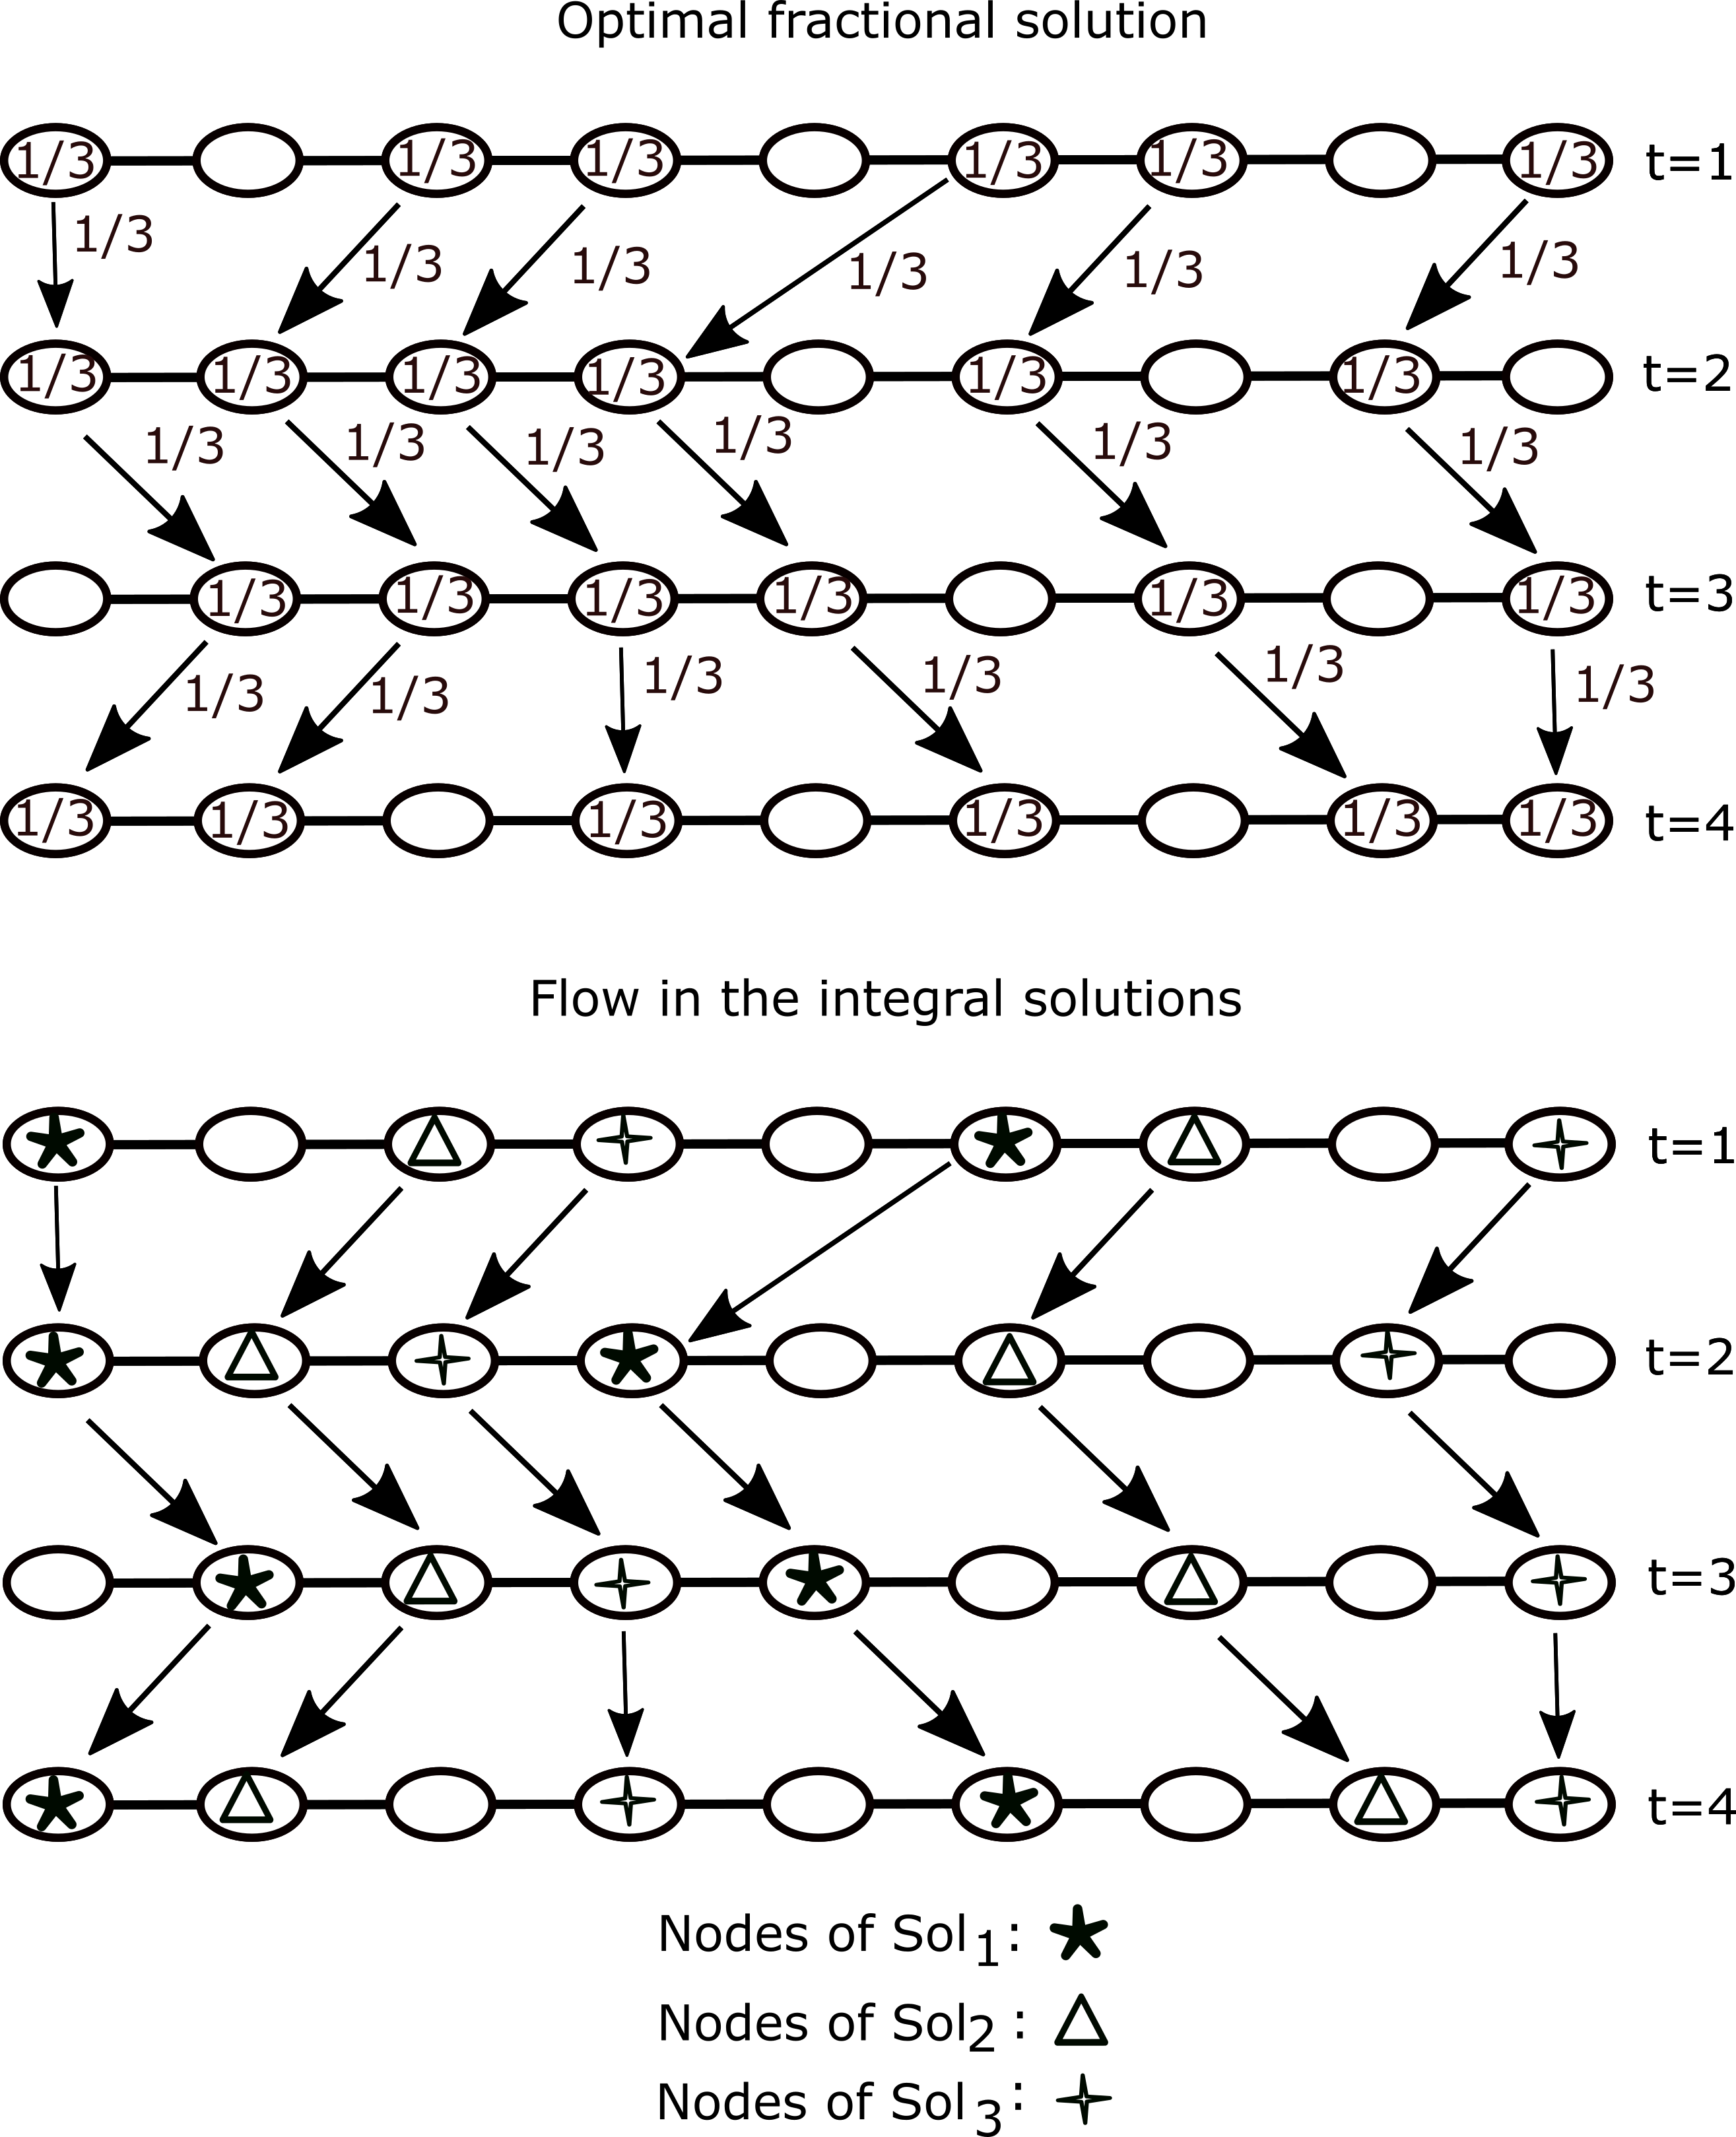
\includegraphics[scale=0.15]{moving_cost.png}
%     \caption{In this example, we illustrate the relation of the integral solutions $\Sol_p$ with an optimal fractional solution in terms of moving facilities. We have 2 facilities ($K=2$) and $N=3$. On the top, we depict an instance where the optimal fractional solution $\ZLP$ has placed $1/N=1/3$ amount of facility on some nodes in the path. We show in Lemma~\ref{l:moving_cost} that $\ZLP$ sends these positive fractions of facilities to nodes of the next stage as depicted by the arrows. The figure on the bottom illustrates how $\Sol_1, \Sol_2$ and $\Sol_3$ move facilities between stages. Observe that each facility is moved to the same node that has moved it's fraction in $\ZLP$}
%     \label{fig:movingcost}
% \end{figure}

\begin{lemma}\label{l:moving_cost}
For a facility $k$ at stage $t$, under Assumption~\ref{a:1} it holds that

\[
\frac{1}{N}\sum_{p=1}^N \MovC(\Sol_p) = \sum_{t=1}^T\sum_{k\in F} S_k^t.
\]
\end{lemma}
\begin{proof2}
By Assumption~\ref{a:1}, $c_j^t=1/N$ if $j\in V_t^+= \{Y_1^t,\ldots,Y_{KN}^t\}$
and $0$ otherwise. Notice that the connection cost of the optimal fractional 
solution only depends on the
variables $c_j^t$. As a result, $f_{k j}^t,S_k^t,S_{k j l}^t$ must be the optimal 
solution of the following linear program.


\begin{equation}\label{eq:LP1}
\begin{array}{ll@{}ll}
\text{minimize}  &  \sum \limits_{t=1}^{T}\sum \limits_{k=1}^KS_k^t\\
& \\
\text{s.t.}& \sum\limits_{k \in [K] }f^t_{kj}=\frac{1}{N}   & \,\,\,\,\,\,\,\, \forall j \in V_t^+,t\in [T] 
\\
        &\sum \limits_{j \in V_t^+} f_{kj}^t=1 & \,\,\,\,\,\,\,\, \forall k\in [K], t \in [T]\\
        &S_k^t = \sum \limits_{j,l \in V} d(j,l)S_{kjl}^t & \,\,\,\,\,\,\,\, \forall k \in [K], t\in [T] \\
        &\sum \limits_{j \in V_{t-1}^+} S_{kjl}^t =f_{kl}^t 
        & \,\,\,\,\,\,\,\, \forall k \in [K],l \in 
        V_t^+,t\in [T]\\
        &\sum \limits_{l \in V_t^+} S_{kjl}^t = f_{kj}^{t-1} 
        & \,\,\,\,\,\,\,\, \forall k \in [K],j \in 
        V_{t-1}^+,t\in [T]\\
\end{array}
\end{equation}
\medskip

\noindent We can relax the linear program above (\ref{eq:LP1}) to get the more convenient linear program that follows. 
\begin{equation}\label{eq:LP2}
\begin{array}{ll@{}ll}
\text{minimize}  &  \sum \limits_{t=1}^T\sum \limits_{j \in V_{t-1}^+,l \in V_t^+} 
d(j,l)F_{jl}^t\\
& \\
\text{s.t.}& \, \sum\limits_{l \in V_t^+}F^t_{jl}=\frac{1}{N}   & \forall j \in V_{t-1}^+,t\in 
[T] \\
& \sum \limits_{j \in V_{t-1}^+} F^t_{jl}=\frac{1}{N} & \forall l\in V_t^+, t\in [T] \\
\end{array}
\end{equation}
\medskip

\noindent
It is easy to prove that the LP~(\ref{eq:LP2}) is a relaxation of LP~(\ref{eq:LP1})
by setting $F_{jl}^t = \sum _{k \in F}S_{kjl}^t$. Moreover, the above LP 
describes a flow 
problem between the nodes $V_t^+$, where $F_{jl}^t$ is the amount of flow 
going from node $j \in V_{t-1}^+$
to node $l \in V_t^+$ (see Figure~\ref{f:flow}).

Next, we proceed to the final step of our proof. First, observe that 
$F^t_{Y_j^{t-1}Y_j^t}$ is feasible
solution for the above LP since $|V_{t-1}^+|=|V_t^+|=K\cdot N$. If we prove that 
this assignment minimizes the objective, then we are done. Assume that in an  
optimal solution, $F^t_{Y_1^{t-1}Y_1^t}<1/N$. 
Since $\sum\limits_{l \in V_t^+} F^t_{Y_1^{t-1}l}=\frac{1}{N}$,
there exists $Y_j^{t}$ such that $F^t_{Y_1^{t-1}Y_j^{t}}>0$. Similarly, by using 
the second constraint we obtain that 
$F^t_{Y_{j'}^{t-1}Y_1^{t}}>0$. Let $\epsilon = 
\min(F^t_{Y_1^{t-1}Y_j^{t}},F^t_{Y_{j'}^{t-1}Y_1^{t}})$. Observe that if we 
increase $F^t_{Y_1^{t-1}Y_1^{t}}$, $F^t_{Y_{j'}^{t-1}Y_j^{t}}$ by $\epsilon$ and 
decrease $F^t_{Y_1^{t-1}Y_j^{t}}$, $F^t_{Y_{j'}^{t-1}Y_1^{t}}$ 
by $\epsilon$, we obtain another feasible solution. The cost difference of the 
two solutions is
$D=\epsilon (d(Y_1^{t-1},Y_j^{t}) + d(Y_{j'}^{t-1},Y_1^{t}) - d(Y_1^{t-1},Y_1^{t}) - 
d(Y_{j'}^{t-1},Y_j^{t}))$. If we prove that $D$ is
non-negative, we are done. We show the latter using the fact that $Y_1^{t-1} \leq 
Y_{j'}^{t-1}$ and $Y_1^{t} \leq Y_j^{t}$. More precisely,
\begin{itemize}
 \item If $Y_1^{t-1} \leq Y_1^{t}$ then $D\geq 0$ since $Y_1^{t} \leq Y_j^{t}$.
 \item If $Y_1^{t-1} \geq Y_1^{t}$ then $D\geq 0$ since $Y_1^{t-1} \leq 
 Y_{j'}^{t-1}$.
\end{itemize}

Until now, we have shown that in the optimal solution, the node $Y_1^{t-1}$ 
sends all of her flow to the node $Y_1^{t}$. Meaning that
$Y_1^{t}$ does not receive flow by any other node apart from $Y_1^{t-1}$. By 
repeating the same argument,
it follows that in the optimal solution each node $Y_j^{t-1}$ sends all of her flow 
to $Y_j^{t}$. Thus, we have that
\begin{equation}\label{eq:mov_cost}
\frac{1}{N}
\sum\limits_{t=1}^T \sum_{j=1}^{K \cdot N} \dist(Y^{t-1}_j,Y^t_j)=
\sum_{t=1}^T\sum_{k\in F} S_k^t.
\end{equation}
We can see an illustration of the previous arguments below:
\tikzstyle{vertex}=[circle,fill=black!25,minimum size=27pt,inner sep=0pt]
\tikzstyle{weight} = [font=\small,above=0pt]
\tikzstyle{weight2} = [font=\small,above=4pt,left=9pt]
\tikzstyle{weight3} = [font=\small,below=5pt,left]
\tikzstyle{weight4} = [font=\small,below=10pt,left]
\tikzstyle{weight5} = [font=\small,below]
\tikzstyle{weight6} = [font=\small,above=12pt]

\tikzstyle{edge} = [draw,thick,->]
\usetikzlibrary{calc,arrows.meta,positioning}


\begin{figure}[ht] 
\centering	
\begin{tikzpicture}[scale=0.72]
\node[vertex] (1) at (0,0) {$Y_1^0$};
\node[vertex] (2) at (0,-1.5) {$Y_2^0$};
\node[vertex] (3) at (0,-5) {$Y_{K\cdot N}^0$};
\node at ($(2)!.5!(3)$) {\vdots};
\node[vertex] (4) at (3,0) {$Y_1^1$};
\node[vertex] (5) at (3,-1.5) {$Y_2^1$};
\node[vertex] (6) at (3,-5) {$Y_{K\cdot N}^1$};
\node at ($(5)!.5!(6)$) {\vdots};

\node[vertex] (10) at (6,0) {$Y_1^{t-1}$};
\node[vertex] (11) at (6,-2.25) {$Y_{j'}^{t-1}$};
\node[vertex] (12) at (6,-5) {$Y_{K\cdot N}^{t-1}$};
\node at ($(11)!.5!(12)$) {\vdots};
\node[vertex] (13) at (9,0) {$Y_1^t$};
\node[vertex] (14) at (9,-3) {$Y_j^t$};
\node[vertex] (15) at (9,-5) {$Y_{K\cdot N}^t$};
\node at ($(14)!.5!(15)$) {\vdots};

\node at ($(4)!.5!(10)$) {\ldots};
%\node at ($(5)!.5!(11)$) {\ldots};
\node at ($(6)!.5!(12)$) {\ldots};
 \path[edge] (10) -- node[weight] {$F_{Y_1^{t-1}Y_1^t}^t$} (13);
 \path[edge] (10) -- node[weight6] {$F_{Y^{t-1}_1Y^t_j}^t$} (14);
 
  \path[edge] (11) -- node[weight4] {} (13);
 \path[edge] (11) -- node[weight5] {$F_{Y^{t-1}_{j'}Y^t_j}^t$} (14);
 \path[edge] (2) -- node[weight] {} (5);
 \path[edge] (1) -- node[weight] {$F_{Y^{t-1}_{1}Y^t_1}^t$} (4);
 \path[edge] (1) -- node[weight] {} (5);
 \path[edge] (2) -- node[weight2] {$F_{Y^{t-1}_{2}Y^t_1}^t$} (4);
 \path[edge] (3) -- node[weight] {} (6);

 \node[vertex] (20) at (12,0) {$Y_1^{T-1}$};
\node[vertex] (21) at (12,-1.5) {$Y_2^{T-1}$};
\node[vertex] (22) at (12,-5) {$Y_{K\cdot N}^{T-1}$};
\node at ($(21)!.5!(22)$) {\vdots};
\node[vertex] (23) at (15,0) {$Y_1^T$};
\node[vertex] (24) at (15,-1.5) {$Y_2^T$};
\node[vertex] (25) at (15,-5) {$Y_{K\cdot N}^T$};
\node at ($(24)!.5!(25)$) {\vdots};

\node at ($(13)!.5!(20)$) {\ldots};
%\node at ($(14)!.5!(21)$) {\ldots};
\node at ($(15)!.5!(22)$) {\ldots};

 \path[edge] (20) -- node[weight] {} (24);
 \path[edge] (20) -- node[weight] {$F_{Y_1^{T-1}Y_1^{T}}^T$} (23);
 \path[edge] (21) -- node[weight] {} (24);
 \path[edge] (21) -- node[weight2] {} (23);
 \path[edge] (22) -- node[weight] {} (25);
%\node at ($(6)!.5!(12)$) {\ldots};
\node at ($(10)!.5!(11)$) {\vdots};
\node at ($(13)!.5!(14)$) {\vdots};
\path[edge] (12) -- node[weight] {} (15);
\end{tikzpicture}

\caption{The flow described by LP~(\ref{eq:LP2}).} \label{f:flow}
\end{figure}


\noindent
Finally, by the definition of the solutions $\Sol_p$ we have that:

\begin{align*}
\frac{1}{N}\sum\limits_{p=1}^N \MovC(\Sol_p) &= 
\frac{1}{N}
\sum\limits_{p=1}^N \sum\limits_{t=1}^T \sum_{m= 1}^K \dist(Y^{t-1}_{(m-1)N + 
p},Y^t_{(m-1)N + p})\\
&=
\frac{1}{N}
\sum\limits_{t=1}^T \sum_{m=1}^K\sum\limits_{p=1}^N 
\dist(Y^{t-1}_{(m-1)N+p},Y^t_{(m-1)N+p})\\
&= 
\frac{1}{N}
\sum\limits_{t=1}^T \sum_{j=1}^{K \cdot N} \dist(Y^{t-1}_j,Y^t_j)\\
&=
\sum_{t=1}^T\sum_{k\in F} S_k^t,
\end{align*}

where the the last equality follows from equation~\ref{eq:mov_cost}.
\end{proof2}
\medskip

The previous lemma concludes the proof of Theorem~\ref{l:main_stageing} under Assumption~\ref{a:1}. In the next section, we show how to prove Theorem~\ref{l:main_stageing} in the general case.







\subsection{Proving Theorem~\ref{l:main_stageing} in the General Case} \label{s:rounding_general}
In this section, we prove Theorem~\ref{l:main_stageing}
in the general case.
% we present the proof details to show that an optimal fractional solution for the $\text{LP}_{\text{Reallocation}}$ has the same cost with the solution provided by Algorithm~\ref{alg:offline} even without satisfying Assumption~\ref{a:1}.
This will be achieved in the following steps:
\begin{enumerate}
    \item From an optimal fractional  solution $\ZLP$ for the original path $P$, we will construct an optimal fractional solution $\ZLPO$ for a path $P'$ that satisfies Assumption~\ref{a:1}.
    \item We will show that $\ZLP$ and $\ZLPO$ have the same cost.  
    \item We will define integral solutions $\Sol_p^*$ (see Definition~\ref{d:Integral_original}) in $P$ that correspond to the integral solutions $\Sol_p$ in $P'$ that satisfy Assumption~\ref{a:1}.
    \item The solution provided by Algorithm~\ref{alg:offline} is one of the solutions $\Sol_p^*$.
\end{enumerate}


We begin by constructing an optimal fractional solution that satisfies Assumption~\ref{a:1} from a generic optimal fractional solution. As already discussed, Assumption~\ref{a:1} is 
not satisfied in general by a fractional solution of the relaxation of the $\LPR$~(\ref{LP_Reallocation}).
Each $S_{k j \ell}^t$ will be either $0$ or $A_{k j \ell}^t/N_{k j \ell}^t$, for  
some positive integers $A_{k j \ell}^t, N_{k j \ell}^t$. However, each positive $f_{kj}^t$ 
has the form $B_{k j}^t/N$,  where $N = \Pi_{S_{kj\ell}^t > 0} N_{k j \ell}^t$. 
This is due to the constraint $f_{k j}^t = \sum_{j \in V}S_{k j \ell}^t$.

Now, consider the path $P' = (V',E')$ constructed from
path $P= (V,E)$ as follows: Each node $j \in V$
is split into $K N$ copies $\{j_1,\ldots, j_{KN}\}$ with zero distance 
between them. Consider also the $\LPR$~(\ref{LP_Reallocation}), when the underlying path is $P' = 
(V',E')$ and at each stage $t$, each agent $i$ is located
at a node of $V'$ that is a copy of $i$'s original location, $\Loc'(i,t) = \ell 
\in V'$, where $\ell \in \text{Copies}( \Loc(i,t))$.
Even though paths $P$ and $P'$ form two different linear programs, these linear programs  are closely related since a solution 
for one can be converted to a solution for the other with the exact same 
cost. This is due to the fact that
for all $j,h \in V$, $\dist(j,h) = \dist(j',h')$, where $j'\in \text{Copies}(j)$ and $h'\in 
\text{Copies}(h)$. 

% The reason that we defined $P'$ and the second LP is the following: Given an 
% optimal fractional solution of the LP defined for $P$, we construct a 
% fractional solution for the LP defined for $P'$ with the exact same cost, which 
% additionally satisfies Assumption~\ref{a:1}. Thus, we can obtain $N$ integral solutions for $P'$ with average cost equal the optimal fractional cost. These integral solutions 
% for $P'$ can be easily converted to integral solutions for $P$, thus proving the statement of   
% Theorem~\ref{l:main_stageing}. 



Given the fractional positions $\{f_{k j}^t\}_{t \geq 1}$ of an optimal solution of 
the LP formulated for $P=(V,E)$, we construct the fractional positions
of the facilities in $P' = (V',E')$ as follows: 
If $f_{k j}^t = B_{k j}^t / N$, then 
facility $k$ puts a $1/N$ amount of facility in $B_{k j}^t$ nodes of the set 
$\text{Copies}(j)=\{j_1,\ldots, j_{K N}\}$
that have a $0$ amount of facility. The latter is possible since there are exactly 
$K N$ copies of each $j \in V$ and $c_j^t \leq K$ (that is the reason we 
required $KN$ copies of each node). The values for the rest of the variables are 
defined in the proof of the following lemma.

\begin{figure}
    \centering
    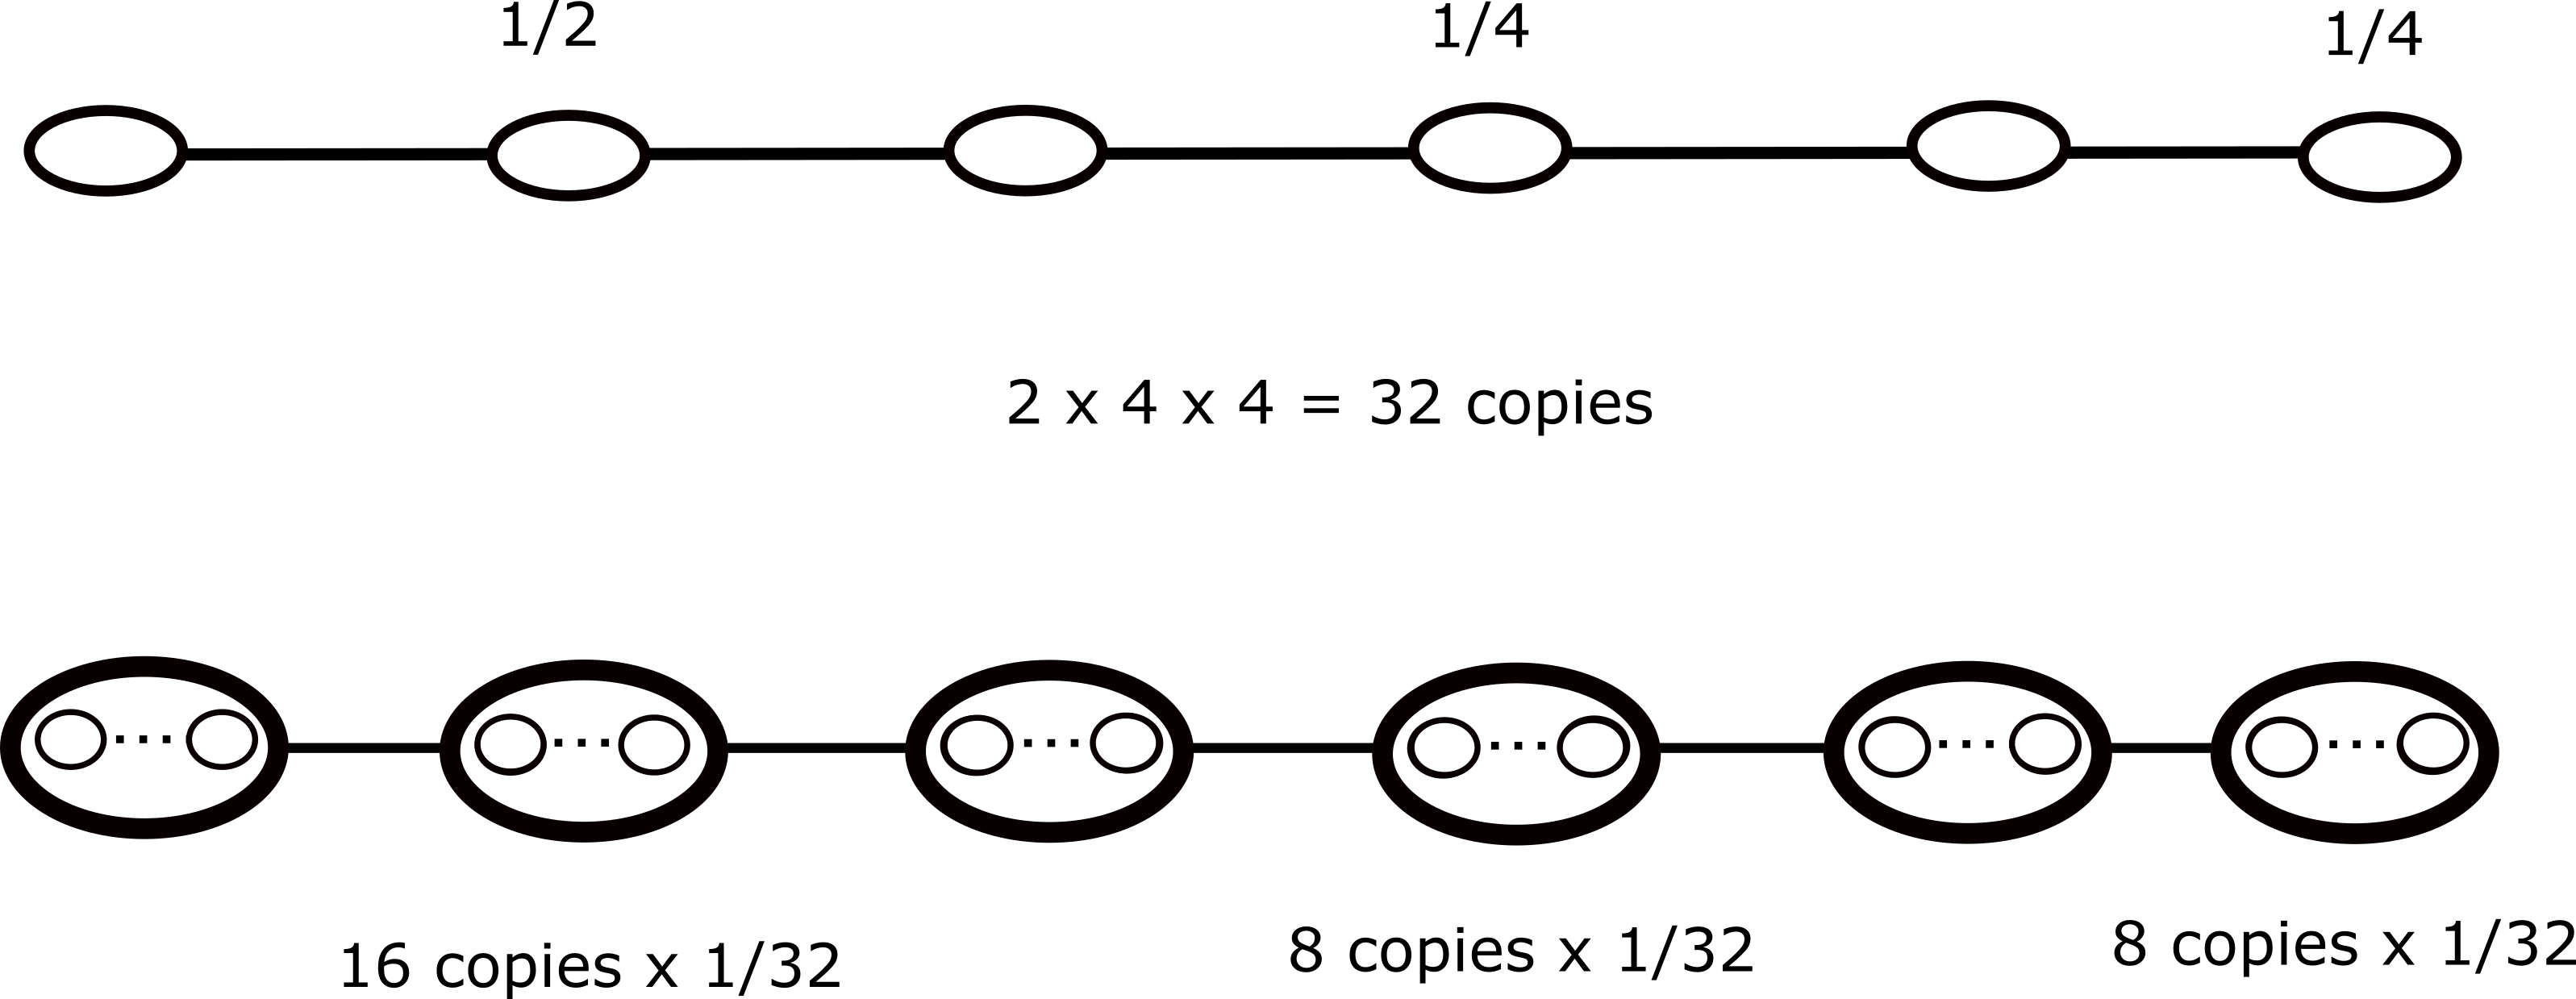
\includegraphics[scale=0.14]{chapters/previous_work/general.png}
    \caption{In this figure, we see on the top a fractional solution for the original locations path $P$ and on the bottom a fractional solution for the path $P'$ under Assumption~\ref{a:1}. The instance has one facility ($K=1$). In $P$, we have an amount of $c_j^t=1/2$ on the second node from the left and an amount of $c_j^t=1/4$ on the fourth and sixth node on the left. Therefore $N=2 \cdot 2 \cdot 4=32$ and each node of $P$ splits in $32$ copies with zero distance in $P'$. Thus, in $P'$, we have 16 nodes corresponding to the second node in $P$ with $c_j^t=1/32$, $8$ nodes corresponding to the fourth node in $P$ with $c_j^t=1/32$ and $8$ nodes corresponding to the sixth node in $P$ with $c_j^t=1/32$. Thus, these two solutions have the same cost.
    }
    \label{fig:general}
\end{figure}


\begin{lemma}\label{l:construction}
Let $\{f_{kj}^t, c_j^t, S_{kjl}^t,\zeta_{ij}^t\,  S_k^{t} \}_{t \geq 1}$  be an optimal fractional solution $\ZLP$
for the LP~(\ref{LP_Reallocation}) in the locations path $P$.
Then, there exists a solution $\ZLPO=\{f_{k j}^{'t}, c_j^{'t}, S_{k j l}^{'t},\zeta_{ij}^{'t},S_k^{'t} 
\}_{t \geq 1}$
of the LP~(\ref{LP_Reallocation}) in the path $P'$ such that:
\begin{itemize}
    \item $\Cost(\ZLPO)$= $\Cost(\ZLP)$ \,\,\, \, \,\,\,\, \, \,\,\,\, \, \,\, \,\, (1)

    \item $f^{'t}_{k\ell} = 1/N$ or $0$,  for each $\ell \in V'$ \,\,\, \, \, \,(2)

    \item $c^{'t}_{\ell} = 1/N$ or $0$,  for each $\ell \in V'$ \, \, \, \,\,  \,(3)
    
    \item $c^t_j = \sum\limits_{\ell \in \text{Copies}(j)}c^{'t}_{\ell}$,  for each $j \in 
    V'$ \, \, \,(4)
\end{itemize}
\end{lemma}
\begin{proof2}
We start by setting values to the variables $f_{kj}^{'t}$.
Initially, all $f_{kj}^{'t} = 0$.
We know that if $f_{kj}^t>0$, then it equals $B_{kj}^t/N$,
for some positive integer $B_{kj}^t$. For each
such $f_{kj}^t$, we find $u_1,\ldots,
u_{B_{kj}^t} \in \text{Copies}(j)$ with $f_{ku_h}^{'t} = 0$. Then, we set 
$f_{k u_h}^{'t} = 1/N$ for $h = \{1, \ldots ,B_{kj}^t\}$. Since there are $KN$ copies of 
each node $j \in V$ and $\sum_{j \in V}f_{kj}^t \leq K$, we can always find 
sufficient copies of
$j$ with $f_{ku}^{'t} = 0$. When this step is terminated, we are sure that 
conditions $2,3,4$ are satisfied. 

We continue with the variables $S_{kj\ell}^{'t}$.
Initially, all $S_{kj\ell}^{'t} = 0$. Then, each positive
$S_{kj\ell}^{t}$ has the form $B_{kj\ell}^{t}/N$.
Let $B = B_{kj\ell}^{t}$ to simplify notation.
We now find $B$ copies of $u_1,\ldots, u_{B}$ of $j$ and $v_1,\ldots, v_B$ of 
$\ell$ so that

\begin{itemize}
    \item $f_{ku_1}^{' t} = \ldots = f_{ku_{B}}^{'t} = f_{kv_1}^{'t} = \ldots = 
    f_{kv_{B}}^{'t} = 1/N$.

 \item $S_{ku_1 h }^{'t} = \ldots = S_{k u_{B} h}^{'t} = S_{k h v_1 }^{'t} = \ldots = 
 S_{k h v_{B}}^{'t} = 0$
for all $h \in V'$.

\end{itemize}
We then set 
$S_{ku_1 v_1 }^{'t} = \ldots = S_{ku_B v_B }^{'t} = 1/N$. Since $\sum 
_{\ell \in V}S_{kj \ell }^{t} = f_{kj}^t$ and $\sum _{j \in V}S_{kj \ell }^{t} = 
f_{k\ell}^t$, we can always find $B_{kj\ell}^t$ pairs of copies of $j$ and $\ell$ that 
satisfy the above requirements. We can now prove that the movement cost
of each facility $k$ is the same in both solutions.
\begin{align*}
\sum_{j \in V}\sum_{\ell \in V}\dist(j,\ell)S_{kj\ell}^t &=
\sum_{j \in V}\sum_{\ell \in V}\dist(j,\ell)B_{kj\ell}^t/N\\
&=
\sum_{j \in V}\sum_{\ell \in V}\sum_{h \in \text{Copies}(j)}\sum_{ h' \in 
\text{Copies}(\ell)}S_{k h h'}^{'t}\dist(h,h')\\
&=
\sum_{j' \in V'}\sum_{\ell' \in V'} S_{k j' \ell'}^{'t}\dist(j',\ell').
\end{align*}
\noindent The second equality follows from the fact that $h$ and $h'$ are copies of 
$j$ and $\ell$ respectively and thus 
$\dist(h,h')=\dist(j,\ell)$.

Finally, set values to the variables $\zeta_{ij}^{'t}$ for each $j \in V'$. Again, each 
positive $\zeta_{ij}^t$ equals
$B_{ij}^t/N$, for some positive integer. We take $B_{ij}^t$ copies of $j$, 
$u_1,\ldots,u_{B_{ij}^t}$ and
set $\zeta_{iu_1}^{'t} = \ldots = \zeta_{iu_{B_{ij}^t}}^{'t} = 1/N$. The connection cost of 
each agent $i$ remains the same since 

\begin{eqnarray*}
\sum_{j \in V} \dist(\Loc(i,t),j)\zeta_{ij}^t &=&
\sum_{j \in V} \dist(\Loc(i,t),j)B_{ij}^t/N\\
&=&
\sum_{j \in V} \dist(\Loc(i,t),j)\sum_{j' \in \text{Copies}(j)}\zeta_{i j'}^{'t}\\
&=&
\sum_{j \in V} \sum_{j' \in \text{Copies}(j)}
\dist(\Loc'(i,t),j') \zeta_{i j'}^{'t}\\
&=&
\sum_{h \in V'} \dist(\Loc'(i,t),h) \zeta_{i h}^{'t},\\
\end{eqnarray*}
where the third equality holds since $\Loc'(i,t) \in \text{Copies}(\Loc(i,t))$.
\end{proof2}



% The key point is that the produced solution $\{f_{k \ell}^{'t},c_{j}^{'t}
% ,S_{k j \ell}^{'t}, x_{i j}^{'t},S_k^{'t}\}$

% will satisfy the following properties (see Lemma~\ref{l:construction}):

% \begin{itemize}
%     \item its cost equals $\Z_{LP}^*$

%     \item $f^{'t}_{k\ell} = 1/N$ or $0$, for each $\ell \in V'$

%     \item $c^{'t}_{\ell} = 1/N$ or $0,$ for each $\ell \in V'$
    
%     \item $c^t_j = \sum\limits_{\ell \in \text{Copies}(j)}c^{'t}_{\ell}$,  for each $j \in 
%     V$
% \end{itemize}

\medskip

\noindent
Before, we move to the proof of our main result, we give the formal definition of the integral solutions $\Sol_p^*$ for the original path $P$ (these are referred as $\Sol_p$ in Theorem~\ref{l:main_stageing}).

\begin{definition}\label{d:Integral_original}
$\Sol_p^*$ denotes the integral solution in the original positions path $P$ that corresponds to the solution $\Sol_p$ of path $P'$. That is, if $\Sol_p^*$ places the $m$th facility to a node $j \in V$ in $P$, then $\Sol_p$ places the $m$th facility to a node $j_c$ in $P'$ that is one of the copies of $j$, namely $j_c \in \mathrm{Copies}(j)$.

\end{definition}
To conclude this section, we prove Theorem~\ref{l:main_stageing}.

\begin{proof}[Proof of Theorem~\ref{l:main_stageing}]
By Lemma~\ref{l:construction}, an optimal fractional solution $\ZLPO$ for $P'$ satisfies Assumption~\ref{a:1}. Applying Lemma~\ref{l:connection_cost} for $\ZLPO$, we get $N$ integral solutions $\Sol_p$ for $P'$, which place the $m$th facility to the $(m-1)N + p,$ $1\leq p\leq N$, node of $V^{+}_t$ 
($Y^{t}_{(m-1)N + p} \in V'$) such that  
\[\frac{1}{N}\sum_{p=1}^N \ConC^t_i(\Sol_p) =\sum_{j\in V'} 
\dist(\Loc(i,t),j)\zeta_{ij}^{'t}
\]
where the right hand side of the equality is the connection cost for the fractional solution $\ZLPO$ in $P'$. By Lemma~\ref{l:construction} the connection cost of the solution $\ZLPO$ for $P'$ equals the connection cost of an optimal fractional solution $\ZLPO$ for the original path $P$. By Definition~\ref{d:Integral_original}, the integral solution $\Sol_p^*$  places facility $m$, $1 \leq m \leq K$, on a node in $P$ which has zero distance from the node that the integral solution $\Sol_p$ places the facility $m$.   
Thus, we have $N$ integral solutions $\Sol_p^*$ for 
$P$, such that
% which
% place the $m$th facility to the node $j_{m,p}^t \in V$, such that
% $Y^{'t}_{(m-1)N + p} \in \text{Copies}(j_{m,p}^t)$,
\[\frac{1}{N}\sum_{p=1}^{N} \ConC^t_i(\Sol_p^*) =\sum_{j\in V} 
\dist(\Loc(i,t),j)\zeta_{ij}^t
.\]

This proves the first claim (1) of Theorem~\ref{l:main_stageing}. Using the same arguments and  Lemma~\ref{l:moving_cost}, we can prove that the average moving cost of the solutions $\Sol_p^*$ equals the moving cost of the optimal fractional solution $\ZLP$.
% the $N$ integral solutions for $P'$ that place the $m$th facility to the $(m-1)N + p,$ $1\leq p\leq N$, node of $V^{'+}_t$ 
% ($Y^{'t}_{(m-1)N + p} \in V'$) have average moving cost $\MovC(\Z_{LP}^*)$. So the $N$ integral solutions for 
% $P$ that
% place the $m$th facility to the node $j_{m,p}^t \in V$, such that
% $Y^{'t}_{(m-1)N + p} \in \text{Copies}(j_{m,p}^t)$, have again average cost $\MovC(\Z_{LP}^*)$. 
Thus, both claims Theorem~\ref{l:main_stageing} hold. Finally, it is easy to see that the solution provided by Algorithm~\ref{a:1} corresponds to $\Sol_1^*$, 
thus is one of the integral solutions for $P$ and this concludes the proof of Theorem~\ref{l:main_stageing}.
% puts the facility to the node $j_{m,1}^t \in V$, such that
% $Y^{'t}_{(m-1)N + 1} \in \text{Copies}(j_{m,1}^t)$, 
\end{proof}